\documentclass{article}
\usepackage{icml2026}

% ------------------------------------------------------------
% Packages
% ------------------------------------------------------------
\usepackage[utf8]{inputenc}
\usepackage{amsmath,amssymb,amsthm,amsfonts}
\usepackage{algorithm}
\usepackage{algorithmic}
\usepackage{graphicx}
\usepackage{wrapfig}
\usepackage{subcaption}
\usepackage{booktabs}
\usepackage{float}
\usepackage{placeins}
\usepackage{natbib}
\usepackage{enumitem}
\usepackage{mathtools}
\usepackage{tikz}
\usepackage{pgfplots}
\usepackage{fontspec}
\usepackage[english,provide=*]{babel}
\usepackage{changepage}
\usepackage{pgfplots}
\usepgfplotslibrary{groupplots}
\usepackage{pgfplotstable}

\usepackage{hyperref}
\usepackage{url}
\usepackage{natbib}

\pgfplotsset{compat=1.18}

% ------------------------------------------------------------
% Theorem environments
% ------------------------------------------------------------
\newtheorem{theorem}{Theorem}
\newtheorem{proposition}{Proposition}
\newtheorem{lemma}{Lemma}
\newtheorem{remark}{Remark}

% ------------------------------------------------------------
% Macros
% ------------------------------------------------------------
\babelprovide[import,onchar=ids fonts]{english}
\babelprovide[onchar=ids fonts]{tifinagh}
% Standard Latin Modern is the default for fontspec if no other font is set.
% We only define the font for Tifinagh.
\babelfont[tifinagh]{rm}{Ebrima}

% Robust \yat definition with fallback
\newfontfamily\tifinaghfont{Noto Sans Tifinagh}
\DeclareRobustCommand{\E}{\text{\normalfont\tifinaghfont ⵟ}}

\newcommand{\R}{\mathbb{R}}
\newcommand{\Sph}{\mathbb{S}}
\newcommand{\norm}[1]{\left\lVert #1 \right\rVert}
\newcommand{\inner}[2]{\left\langle #1, #2 \right\rangle}

% ------------------------------------------------------------
% Title / Authors
% ------------------------------------------------------------

\begin{document}

\twocolumn[
\icmltitle{SLAY:\\
Geometry-Aware Spherical Linearized Attention with Yat-Kernel}
\icmltitlerunning{SLAY: Geometry-Aware Spherical Linearized Attention with Yat-Kernel}

\begin{icmlauthorlist}
\icmlauthor{Jose Miguel Luna}{equal}
\icmlauthor{Taha Bouhsine}{equal}
\icmlauthor{Krzysztof Choromanski}{}
\end{icmlauthorlist}

\icmlaffiliation{equal}{Anonymous Institution}
\icmlcorrespondingauthor{Anonymous}{anon.email@domain.com}

\icmlkeywords{Linear Attention, Neural Matter Networks, Random Features, Long Context}

\vskip 0.3in
]

\printAffiliationsAndNotice{}

% ------------------------------------------------------------
% Abstract
% ------------------------------------------------------------
\begin{abstract}
We propose a new class of linear-time attention mechanisms, relying on the relaxed, computationally-efficient version of the recently introduced \emph{\E-Product}, often referred to as the Yat-kernel \citep{bouhsine2025no}, yielding geometry-aware interactions and inspired by the inverse-square interactions in Physics. Our introduced \emph{Spherical Linearized Attention with YAT-Kernels}, or \emph{SLAY}, constrains queries and keys to the unit sphere so the kernel depends only on the angular alignment. Using Bernstein’s Theorem, we express the spherical YAT-kernel as a nonnegative mixture of polynomial--exponential product kernels and derive a strictly positive random-feature approximation with linear-time $O(L)$ attention, where $L$ stands for the sequence length. We prove positive definiteness and boundedness on the sphere and show that the estimator yields nonnegative scores with a positive denominator under mild conditions. Empirically, SLAY matches full spherical YAT attention and compares favorably to linearized baselines on language and vision tasks, while retaining linear scaling in $L$.
\end{abstract}

% ============================================================
% 1. Introduction
% ============================================================
\section{Introduction \& Related Work}
\label{sec:intro}

Transformer models \citep{transformers-base, vit, bert, brown, longt5, bigbird} owe much of their success to the \textit{attention mechanism}, which enables dynamic, content-dependent interactions between tokens. In standard Transformers, attention is implemented via softmax operation applied to pairwise query--key similarities. While expressive, it requires constructing explicit $L \times L$ attention matrices for $L$-length input sequences, resulting in quadratic in $L$ time and space complexity. This cost rapidly becomes prohibitive as context lengths grow, fundamentally limiting long-context modeling \citep{yaofu}.

To overcome this bottleneck several so-called \textit{efficient-attention} mechanisms, characterized by time complexity sub-quadratic (often linear) in $L$ were proposed.
They leverage a large spectrum of techniques ranging from clustering/hashing \citep{reformer, routing, lsh-transformer, clustr} to approaches casting attention matrix as a kernel matrix and applying techniques based on random features (RFs) \citep{performers, performer2, chefs, dense-exponential, luo, fft-t, arora}. Those mechanisms critically rely on \textbf{positive} RFs, since regular trigonometric mechanisms, that can be derived from the seminal papers on linearizing shift-invariant kernels \citep{random-features, sinks} lead to unstable training.

Despite these advances, softmax attention remains tied to a specific similarity: the exponential of an inner product. This choice conflates alignment and magnitude, and its unbounded growth requires careful normalization and stabilization. These limitations motivate alternative attention kernels that are geometrically grounded, self-regularizing, and compatible with efficient computation, as explored in activation-free architectures \citep{bouhsine2025no}.

\textit{Neural Matter Networks (NMNs)} introduced the \emph{\E-Product}, also referred to as the Yat-kernel \citep{bouhsine2025no}, a kernel operator inspired by inverse-square interactions in physics:
\begin{equation}
\E(\mathbf{q},\mathbf{k}) \overset{\mathrm{def}}{=} \frac{(\mathbf{q}^\top \mathbf{k})^2}{\|\mathbf{q}-\mathbf{k}\|^2 + \epsilon}
\label{eq:eproduct}
\end{equation}
where $\epsilon > 0$ ensures numerical stability. Unlike standard dot-product similarity, the \E-Product explicitly couples two geometric quantities: \emph{alignment} and \emph{proximity}. The squared inner product in the numerator yields an even (sign-symmetric) alignment score, while the inverse-distance denominator penalizes interactions between distant vectors. This ratio yields a self-regularizing response that can suppress irrelevant interactions without requiring explicit activation functions or normalization layers.

From a theoretical perspective, the \E-Product can be viewed as a kernel-like similarity operator. The NMNs, constructed as linear combinations of \E-Product units, are universal approximators on compact domains, despite being entirely activation-free \citep{bouhsine2025no}. In the context of attention, the \E-Product offers a geometry-aware alternative to softmax similarity. It favors tokens that are both aligned and close in representation space. However, the same geometric coupling introduces a computational obstacle: the denominator $\|\mathbf{q}-\mathbf{k}\|_{2}^2 = \|\mathbf{q}\|_{2}^2 + \|\mathbf{k}\|_{2}^2 - 2\mathbf{q}^\top \mathbf{k}$ entangles query and key terms and prevents the factorization required for efficient linear attention. As a result, naive \E-Product attention still requires explicit pairwise interactions and reverts to quadratic complexity. This mirrors the general limitation for non-factorizable kernels that motivates linearization techniques such as those used in Performers and related models \citep{performers, hedgehog, insuhan}.

This paper addresses this limitation for \E-Attention. We show that by constraining queries and keys to lie on the unit sphere and reformulating the resulting kernel using Bernstein’s Theorem, the \E-Product admits a nonnegative mixture representation, involving polynomial--exponential product kernels, that can be approximated by strictly positive random features. This yields a linear-time attention mechanism that preserves the core geometric and self-regulating properties of the \E-Product while enabling scalable long-context Transformers. We refer to our proposed mechanism as: \emph{Spherical Linearized Attention with YAT-Kernels}, or \emph{SLAY}. Empirically, SLAY matches full spherical YAT attention and compares favorably to linearized baselines on regular Transformer tasks, while retaining $O(L)$-scaling. To summarize, SLAY:
\vspace{-2mm}
\begin{itemize}[leftmargin=1.4em]
\item Enforces unit-norm constraints on queries and keys, decoupling alignment and distance.
\vspace{-1mm}
\item Linearizes the spherical \E-product via an integral representation based on Bernstein’s Theorem.
\vspace{-1mm}
\item Approximates the resulting kernel using strictly positive Tensor Product Random Features.
\vspace{-1mm}
\item Achieves linear-time $O(L)$ attention while preserving key theoretical properties of NMNs.
\end{itemize}
\vspace{-2mm}
This paper is organized as follows: (1) in Section \ref{sec:method}, we present SLAY and provide detailed corresponding theoretical insight, (2) in Section \ref{sec:experiments} we test SLAY on various tasks, including language and vision, by comparing quality-wise with the brute-force mechanisms, as well as other efficient attention methods. We also present speed tests. We conclude in Section \ref{sec:conclusion} and provide additional results in the Appendix.

% ============================================================
% 2. Methodology
% ============================================================
\section{SLAY Mechanism}
\label{sec:method}

\subsection{Preliminaries}
\label{sec:preliminaries}
Denote by $\mathbf{Q} \in \mathbb{R}^{L \times d_{QK}}, \mathbf{K} \in \mathbb{R}^{L \times d_{QK}}$ the query- and key-matrix respectively, with rows denoted as follows: $\mathbf{q}_{1},...,\mathbf{q}_{L} \in \mathbb{R}^{d_{QK}}$ and $\mathbf{k}_{1},...,\mathbf{k}_{L} \in \mathbf{R}^{d_{QK}}$. The attention matrix $\mathbf{A}_{\E} \in \mathbb{R}^{L \times L}$ considered in this paper is of the form: $\mathbf{A}_{\E}=[\E(\mathbf{\widehat{q}}_{i},\mathbf{\widehat{k}}_{j})]_{i=1,...,L}^{j=1,...,L}$, where $\widehat{\mathbf{x}}$ denotes the $L_{2}$-normalized version of $\mathbf{x}$. Our goal is to compute the attention action leveraging $\mathbf{A}_{\E}$, that we refer to as \E-attention, with the spherical constraints, without forming the $L\times L$ matrix $\mathbf{A}_{\E}$ of pairwise interactions. We proceed in several steps, summarized below:
\begin{itemize}
\item linearization of the non-factorizable terms induced by denominators in the YAT-kernel formula via a Laplace integral (Bernstein's Theorem),
\item discretization of the resulting nonnegative mixture using Gauss--Laguerre quadrature,
\item approximating resulting kernels with positive random features from \citep{performers},
\item applying standard matrix multiplication re-ordering for the calculations involving obtained low-rank factorized attention matrix.
\end{itemize}

%Throughout this work, we approximate the spherical \E-product %(YAT) kernel itself; normalization is performed via kernel %sums as in linear attention, not via a softmax nonlinearity.

\subsection{Spherical Constraint}

We assume $d \ge 2$ throughout, where spherical isotropy theory applies. We normalize inputs as follows:
\begin{equation}
\widehat{\mathbf{q}} = \frac{\mathbf{q}}{\|\mathbf{q}\|_{2}},
\widehat{\mathbf{k}} = \frac{\mathbf{q}}{\|\mathbf{k}\|_{2}},
\|\widehat{\mathbf{q}}\|_{2}=\|\widehat{\mathbf{k}}\|_{2}=1
\end{equation}
Expanding the denominator of Eq.~\eqref{eq:eproduct} yields:
\begin{align}
\|\widehat{\mathbf{q}}-\widehat{\mathbf{k}}\|_{2}^2 + \epsilon
&= \|\widehat{\mathbf{q}}\|_{2}^2 + \|\widehat{\mathbf{k}}\|_{2}^2 - 2\widehat{\mathbf{q}}^\top \widehat{\mathbf{k}} + \epsilon \\
&= (2+\epsilon) - 2\widehat{\mathbf{q}}^\top \widehat{\mathbf{k}}.
\end{align}
Let $x=\widehat{\mathbf{q}}^\top \widehat{\mathbf{k}}\in[-1,1]$ and $C=2+\epsilon$. After input normalization, the spherical \E-product becomes:
\begin{equation}
\E_{\text{sph}}(\widehat{\mathbf{q}},\widehat{\mathbf{{k}}})
= \frac{x^2}{C-2x}.
\label{eq:spherical}
\end{equation}
Thus, the kernel depends only on angular alignment.

\paragraph{Geometric intuition.}
On the unit sphere $\Sph^{d-1}$, the squared \emph{chordal} distance is defined as follows:
\[
d_{\Sph^{d-1}}(\widehat{\mathbf{q}}, \widehat{\mathbf{k}})^2 = 2(1 - \widehat{\mathbf{q}}^\top \widehat{\mathbf{k}}).
\]
We conclude that the spherical \E-product can be written as a distance-regularized alignment score:
\begin{equation}
\E_{\mathrm{sph}}(\hat q, \hat k) = \frac{(\widehat{\mathbf{q}}^{\top}\widehat{\mathbf{k}})^{2}}{d_{\Sph^{d-1}}(\widehat{\mathbf{q}}, \widehat{\mathbf{k}})^2 + \epsilon}.
\label{eq:geometric}
\end{equation}
Additional discussion (including invariances and the connection to isotropic spherical kernels \citep{schoenberg1942}) is deferred to Appendix~\ref{app:geom}.

\subsection{Integral Linearization}
With spherical constraints in place, our next step is to linearize the factor $\frac{1}{C-2x}$ in the Eq. \ref{eq:spherical} for the spherical \E-product. We will use Bernstein's Theorem for that.

The function $g(y) = 1/y$ is completely monotone on $(0,\infty)$, which by Bernstein's Theorem implies the Laplace representation $1/y = \int_0^\infty e^{-sy}\,ds$ \citep{widder1941laplace,schilling2012}. To apply this identity to our kernel, we substitute $y = C - 2x$ and verify that $y > 0$ for all $x \in [-1,1]$. Since $x \le 1$ and $C=2+\epsilon$, we have $y=C-2x \ge \epsilon > 0$, hence Bernstein's representation applies (see Lemma~\ref{lem:complete-monotone} in Appendix~\ref{app:background}).

We conclude that by invoking the Laplace representation, the spherical \E-product can be re-written as:
\begin{align}
\E_{\text{sph}}(\widehat{\mathbf{q}},\widehat{\mathbf{k}})
&= x^2 \int_0^\infty e^{-s(C-2x)}ds \\
&= \int_0^\infty e^{-sC}\,\Big[x^2 e^{2s x}\Big]\,ds.
\label{eq:integral}
\end{align}
This expresses the spherical \E-product as a positively weighted mixture of product kernels:
namely, a degree-2 polynomial factor $(\widehat{\mathbf{q}}^\top \widehat{\mathbf{k}})^2$ multiplied by an exponential dot-product kernel $e^{2s\,\widehat{\mathbf{q}}^\top \widehat{\mathbf{k}}}$.
Importantly, the factor $x^2$ cannot be absorbed into a \emph{nonnegative} Laplace weight over plain exponentials without introducing signed correction terms (see Appendix~\ref{app:features}).

\subsection{Quadratures and Positive Features}

\subsubsection{Quadrature (Gauss--Laguerre)}

We approximate the integral in Eq.~\eqref{eq:integral} using $R$-point Gauss--Laguerre quadrature. We apply Gauss--Laguerre quadrature after the change of variables $t = Cs$, so that $\int_0^\infty e^{-Cs} h(s)\,ds = \frac{1}{C}\int_0^\infty e^{-t} h(t/C)\,dt$:
\[
\int_0^\infty e^{-sC} h(s)\,ds \;\approx\; \sum_{r=1}^R w_r\, h(s_r),
\]
where $\{t_r,\alpha_r\}_{r=1}^R$ are the standard Gauss--Laguerre nodes and weights for $\int_0^\infty e^{-t}f(t)\,dt$ and
\[
s_r=\frac{t_r}{C},\qquad w_r=\frac{\alpha_r}{C}.
\]
Thus, the $w_r$ already incorporate the $1/C$ factor induced by $t=Cs$. Since $|x| \le 1$, the integrand $h(s) = x^2 e^{2sx}$ is entire and uniformly bounded by $e^{2s}$, ensuring uniform exponential convergence over $x \in [-1,1]$. Such bounds follow from classical results on Gauss--Laguerre quadrature for entire functions of exponential type (see Theorem 3.6.24 in \citep{davis1984,gautschi2004}); for a shapes/implementation summary, see Appendix~\ref{app:impl} and Appendix~\ref{app:quadrature-details}.

\subsubsection{Polynomial and Exponential RFs}
\label{sec:poly-exp-rfs}

\paragraph{Tensor sketches \& beyond for polynomial kernels:}
For the exact polynomial kernel $(\widehat{\mathbf{q}}^\top \widehat{\mathbf{k}})^2$, the explicit feature map $\phi_{\text{poly}}(\mathbf{u}) = \mathrm{vec}(\mathbf{u} \mathbf{u}^\top) \in \R^{d^2}$ yields exact reconstruction:
\[
\langle \phi_{\text{poly}}(\widehat{\mathbf{q}}), \phi_{\text{poly}}(\widehat{\mathbf{k}}) \rangle = (\widehat{\mathbf{q}}^\top \widehat{\mathbf{k}})^2.
\]
Note that vectors produced by $\phi_{\mathrm{poly}}$ maps are $d^{2}$-dimensional. In practice, we reduce dimensionality via standard low-dimensional reduction techniques. We consider TensorSketch \citep{pham2013} as well as three common approximations to the degree-2 polynomial kernel $k_{\text{poly}}(x,y)=(x^\top y)^2$, described formally in Appendix~\ref{app:prelim-poly}: (i) Random Maclaurin (RM) features \citep{karkarnick2012}, (ii) Nystrom features using anchor points \citep{williams2001nystrom}, and (iii) anchor features using squared inner products to fixed anchors.

\paragraph{Anchor features \citep{scholkopf2002learning}.}
Let anchors $\{\mathbf{a}_i\}_{i=1}^P\subset\R^d$ be fixed reference vectors. Anchor features define mapping $\phi$ as follows:
\[
\phi_{\mathrm{anc}}(\mathbf{x}) = \frac{1}{\sqrt{P}}\bigl[(\mathbf{x}^\top \mathbf{a}_i)^2\bigr]_{i=1}^P,
\]
yielding a simple low-rank approximation whose induced inner products are nonnegative. Unlike Nystrom approximations, anchor features do not require inversion/whitening of the anchor Gram matrix and therefore preserve non-negativity of approximate kernel evaluations. Furthermore, they are empirically stable at small feature budgets, and computationally simple ($O(dP)$ per token). Thus, unless stated otherwise, we use \emph{anchor features} as the default polynomial approximation method in SLAY. The multi-scale sweep in Table~\ref{tab:poly-sweep} (Appendix~\ref{app:poly-ablation}) supports this choice.

Table~\ref{tab:poly-approximations} summarizes the trade-offs between various techniques for approximating squared dot-product kernels, highlighting positivity preservation as a key distinction, determining the robustness of the technique. 

\begin{table*}[t]
\centering
\small
\caption{Polynomial kernel approximation options for the kernel $(\mathbf{x}^\top \mathbf{y})^2$. Here $D_p$ denotes the polynomial-feature dimension, and $P$ denotes the number of anchors (when applicable). \emph{Feature cost} is the asymptotic cost of computing the polynomial features for one vector and excludes quadrature/PRF computation, tensor-product fusion/sketching, and the linear-attention contractions; these additional costs drive end-to-end latency in Section~\ref{sec:experiments}.}
\label{tab:poly-approximations}
\begin{tabular*}{\textwidth}{@{\extracolsep{\fill}}lcccc}
\toprule
Method & Dim. & Feature cost & Unbiased? & $\langle\phi(x),\phi(y)\rangle\ge 0$? \\
\midrule
Exact $\mathrm{vec}(uu^\top)$ & $d^2$ & $O(d^2)$ & Yes & Yes \\
TensorSketch \citep{pham2013} & $D_p$ & $\approx O(d + D_p\log D_p)$ & Approx. & No (not guaranteed) \\
Random Maclaurin \citep{karkarnick2012} & $D_p$ & $O(d\,D_p)$ & Yes & No (not guaranteed) \\
Nystrom \citep{williams2001nystrom} & $P$ & $O(d\,P)$ & Approx. & No (not guaranteed) \\
Anchor features (low-rank) \citep{scholkopf2002learning} & $P$ & $O(d\,P)$ & No & Yes \\
\bottomrule
\end{tabular*}
\end{table*}

For the theoretical non-negativity and denominator-positivity guarantees stated later, we require a polynomial component whose induced score estimates are nonnegative (e.g., the exact map, or anchor features). Signed polynomial approximations (TensorSketch, Random Maclaurin) and Nystrom features can yield negative approximate inner products (see Appendix~\ref{app:stability-experiments}) and are therefore treated as accuracy/efficiency baselines rather than positivity-guaranteeing estimators.

% \paragraph{Why the polynomial factor is needed for fidelity.}
% The $x^2$ factor in Eq.~\eqref{eq:integral} is part of the target kernel; removing it yields a different kernel (see Appendix~\ref{app:features}). Retaining the polynomial factor is essential both for kernel fidelity and for positivity guarantees of the resulting attention scores.

\paragraph{Positive Random Features (PRFs).}
To handle the exponential term $e^{2s\,\widehat{\mathbf{q}}^\top \widehat{\mathbf{k}}}$ from Eq. \ref{eq:integral}, we use PRFs for the exponential kernel, proposed in \citep{performers}, applied to the \emph{original normalized vectors} (we refer to them simply as PRFs; note that this is a different mechanisms than features used to approximate squared dot-product kernels, discussed above):
\begin{equation}
\phi_{\text{PRF}}(\mathbf{u}; s)
=
\frac{1}{\sqrt{D}}
\left[
\exp\!\left(\sqrt{2s}\,\omega_i^\top \mathbf{u} - s\right)
\right]_{i=1}^D,
\end{equation}
where $\omega_i \sim \mathcal{N}(0, \mathbf{I}_d)$ are drawn independently.
This construction satisfies:
\[
\mathbb{E}\!\left[
\phi^{\top}_{\text{PRF}}(\hat q; s)
\phi_{\text{PRF}}(\hat k; s) 
\right]
=
e^{2s\,\widehat{\mathbf{q}}^\top \widehat{\mathbf{k}}}
\]
for unit-norm inputs (a standard unbiasedness result for positive random features; see \citep{performers} and Prop.~\ref{prop:prf-unbiased} in Appendix~\ref{app:background}).

\subsubsection{Fusing RFs for Polynomial \& Exponential Kernels}
Since polynomial feature maps and PRFs are applied to vectors (not scalars), we obtain for each scale $r$:
\begin{equation}
\widetilde{\Psi}_r(\mathbf{u})
=
\sqrt{w_r}\,\mathcal{S}\Bigl(\phi_{\text{poly}}(\mathbf{u})\otimes \phi_{\text{PRF}}(\mathbf{u}; s_r)\Bigr),
\end{equation}
where $\mathcal{S}:\R^{D_pD_r}\to\R^{D_t}$ is a (randomized) sketching operator that approximates the tensor-product feature map without explicitly materializing the $D_pD_r$-dimensional Kronecker vector.
We then define $\widetilde{\Psi}(\mathbf{u})$ as the concatenation over $r=1,\dots,R$ (where $R$ stands for the number of quadrature nodes). Conceptually, the target kernel at each quadrature node is the product kernel $(\widehat{\mathbf{q}}^\top \widehat{\mathbf{k}})^2\,e^{2s_r\widehat{\mathbf{q}}^\top \widehat{\mathbf{k}}}$, whose RKHS is the tensor product $\mathcal{H}_{\text{poly}}\otimes\mathcal{H}_{\exp,s_r}$. The sketching operator $\mathcal{S}$ provides a computationally efficient approximation of this tensor-product feature map.

%\begin{adjustwidth}{1.5em}{1.5em}
\begin{remark}[Feature Map Target]
\label{rem:feature-target}
$\widetilde{\Psi}$ targets the \emph{integrand} $k_s(x)=x^2 e^{2sx}$; consequently,
\vspace{-2mm}
\[
\mathbb{E}[\langle \widetilde{\Psi}(\hat q), \widetilde{\Psi}(\hat k) \rangle] \approx \sum_{r=1}^R w_r\,(\hat q^\top \hat k)^2 e^{2s_r\hat q^\top \hat k},
\]
which is a quadrature approximation to Eq.~\eqref{eq:integral}.
\end{remark}
%\end{adjustwidth}

%\begin{adjustwidth}{1.5em}{1.5em}
\begin{remark}[Bias Decomposition]
\label{rem:bias}
$\langle \widetilde{\Psi}(\hat q), \widetilde{\Psi}(\hat k) \rangle$ is unbiased for the discretized (quadrature) kernel, but biased for the true kernel unless $R\to\infty$.
\end{remark}
%\end{adjustwidth}
\vspace{-3.5mm}
\subsection{Linear-Time Attention Computation}

Given query/key tensors $\mathbf{Q},\mathbf{K} \in \R^{L\times d_{QK}}$ and value tensor $\mathbf{V} \in \mathbb{R}^{L \times d_{V}}$, we compute normalized inputs, apply $\Psi$, and use the standard linear-attention reordering of the computations to calculate attention:
\vspace{-2.5mm}
\begin{equation}
\label{eq:lin-att}
\widehat{\mathbf{Y}} = \frac{\widetilde{\Psi}(\mathbf{Q})\big(\widetilde{\Psi}(\mathbf{K})^\top \mathbf{V}\big)}
{\widetilde{\Psi}(\mathbf{Q})\big(\widetilde{\Psi}(\mathbf{K})^\top \mathbf{1}\big)}.
\end{equation}
Note that this normalization is not a softmax; it corresponds to kernel normalization and preserves linear-time computation.
Here the division is applied row-wise (broadcast across the value dimension); in practice we add a small stabilizer $\delta>0$ to the denominator for numerical stability \citep{higham2002}. Concretely, if $\Psi(\mathbf{Q}),\Psi(\mathbf{K})\in\R^{L\times m}$ (feature dimension $m$) and $\mathbf{V}\in\R^{L\times d_{V}}$, then $\Psi(\mathbf{K})^\top \mathbf{V}\in\R^{m\times d_{V}}$, $\Psi(\mathbf{K})^\top\mathbf{1}\in\R^{m\times 1}$, and the denominator is an $L\times 1$ vector broadcast over $d_{V}$. 
Thus attention matrix $\mathbf{A}_{\E}$ is never explicitly materialized and quadratic in $L$ computations are avoided.
The pseudo-code summarizing the forward pass of the SLAY algorithm is presented in Algorithm 1 Box.

\begin{algorithm}[t]
\caption{Spherical \E-Attention Forward Pass}
\begin{algorithmic}[1]
\REQUIRE $\mathbf{Q},\mathbf{K}\in\R^{L\times d_{QK}}, \mathbf{V} \in \mathbb{R}^{L \times d_{V}}$
\STATE Normalize $\mathbf{Q},\mathbf{K}$ to have unit-norm rows.
\STATE Compute polynomial features $\phi_{\text{poly}}(\mathbf{Q}),\phi_{\text{poly}}(\mathbf{K})$ (e.g., anchor features by default).
\FOR{$r=1$ to $R$}
\STATE Compute PRF features $\phi_{\text{PRF}}(\cdot; s_r)$
\STATE Fuse features via sketched tensor product $\widetilde{\Psi}_r$
\ENDFOR
\STATE Concatenate features $\widetilde{\Psi}(\mathbf{Q}),\widetilde{\Psi}(\mathbf{K})$.
\STATE Compute numerator/denominator as in Eq. \ref{eq:lin-att}.
\RETURN $\widehat{\mathbf{Y}}$
\end{algorithmic}
\end{algorithm}
\paragraph{Complexity Analysis.}
Let $m$ denote the final number of features used in the attention linearization (after concatenating across $R$ quadrature nodes), which in our construction scales as $m=O(RD_t)$. The linear-attention contractions costs $O(L\,m\,d_{V})$ time and $O(L\,m)$ space (the $L\times L$ attention matrix is never formed).
Feature construction depends on the polynomial approximation: exact degree-2 features cost $O(L\,d^2)$, anchor features cost $O(L\,dP)$, Random Maclaurin costs $O(L\,dD_p)$, and TensorSketch costs approximately $O(L\,(d + D_p\log D_p))$ per layer.
The PRF features contribute $O(L\,R\,dD)$ time.
See Appendix~\ref{app:impl} for explicit tensor-product scaling (without sketching) and causal-vs.-non-causal implementation notes.
\vspace{-3mm}
\section{Experiments}
\label{sec:experiments}
We evaluate SLAY along several axes:
\vspace{-3mm}
\begin{itemize}
\item First, we analyze polynomial approximation options to identify optimal configurations for SLAY (see: Sec. \ref{subsec:poly-ablation} for detailed studies).
\vspace{-2mm}
\item Second, we benchmark computational costs by measuring latency, memory, and throughput scaling with sequence length (see: Sec. \ref{subsec:computational-costs}).
\vspace{-2mm}
\item  Third, we evaluate SLAY on \textbf{22} synthetic tasks spanning core capabilities, as well as higher-level behaviors (see: Sec. \ref{subsec:synthetic-experiments}). 
\vspace{-2mm}
\item Fourth, we conduct extreme classification tests to evaluate performance of SLAY versus other attention mechanisms in large-scale classification tasks (see: Sec. \ref{subsec:extreme-classification}). 
\vspace{-2mm}
\item Finally, we test the SLAY mechanism at scale by training and evaluating a series of full-scale Transformer models, varying only the attention mechanism used, leaving every other hyperparameter constant. (see: Sec. \ref{subsec:slayformer}).
\end{itemize}
\vspace{-3mm}
\subsection{Polynomial Factor Approximation}
\label{subsec:poly-ablation}
We isolate the polynomial factor $(\widehat{\mathbf{q}}^\top \widehat{\mathbf{k}})^2$ from the formula of the spherical \E-product (see: Sec. \ref{sec:poly-exp-rfs}) and compare several approximations (anchor, Nystrom, TensorSketch, Random Maclaurin). We report (i) kernel-normalized attention output error relative to exact spherical \E-attention and (ii) forward-pass latency, under matched feature budgets; protocol details and the multi-scale sweep are in Appendix~\ref{app:experiments} and Table~\ref{tab:poly-sweep} (Appendix~\ref{app:poly-ablation}).

For reference, we also include Laplace-only and a Hadamard-fusion variant. These are not polynomial approximations of $(\widehat{\mathbf{q}}^\top \widehat{\mathbf{k}})^2$: they change the estimator by removing or altering the polynomial factor. Under feature-budget matching, they might require substantially larger number of RFs to reach comparable overall feature counts, which can dominate runtime.

\begin{table}[htbp]
\centering
\small
\caption{\small{Kernel approximation quality and latency comparison. Rel.~$\ell_2$ is relative L2 error, Cos is cosine similarity, MSE is mean squared error, and Latency is forward-pass time in milliseconds. For large-scale snapshot, see the ``Large'' block in Table~\ref{tab:poly-sweep}).}}
\label{tab:kernel-combined}
\resizebox{1.05\columnwidth}{!}{%
\begin{tabular}{lcccc}
\toprule
Method & Rel.~$\ell_2\downarrow$ & Cos$\uparrow$ & MSE$\downarrow$ & Latency(ms)$\downarrow$ \\
\midrule
Exact (Spherical) & 0.789 & 0.732 & 1.02e-02 & 5.02 \\
\textbf{Anchor} & \textbf{0.527} & \textbf{0.850} & \textbf{4.55e-03} & \textbf{489.42} \\
Laplace-only & 0.544 & 0.839 & 4.84e-03 & 1905.80 \\
Hadamard (shared $\omega$) & 0.789 & 0.732 & 1.02e-02 & 1932.07 \\
Nystrom & 70.291 & -0.009 & 8.08e+01 & 569.64 \\
TensorSketch & 24823.685 & 0.002 & 1.01e+07 & 547.76 \\
Random Maclaurin & 15826.841 & 0.004 & 4.10e+06 & 551.43 \\
\bottomrule
\end{tabular}%
}
\end{table}

As shown in (Table~\ref{tab:kernel-combined}), anchor and Laplace-only achieve the lowest errors, but anchor is markedly faster (\,$\mathbf{489}$ms vs.~$\mathbf{1906}$ms\,) and thus becomes our default choice in the remaining experiments. Nystrom is substantially less accurate at these budgets. Signed polynomial approximations (TensorSketch and Random Maclaurin) can yield negative approximate inner products, leading to denominator cancellation and severe instability; we include them as efficiency baselines rather than positivity-guaranteeing estimators.

Finally, figure \ref{fig:decision-boundaries} demonstrates the approximation quality of the SLAY anchor kernel, where we observe that SLAY approximates the behavior of the YAT and Spherical YAT kernels remarkably well and at least as well if not better than alternative kernels and their linearized counterparts.

\begin{figure}[htbp]
\centering
\includegraphics[width=\columnwidth]{assets/decision_boundaries.pdf}
\caption{Each panel shows how a kernel partitions the 2D feature space among 5 randomly placed neurons (stars). \textbf{(a)} Linear dot product softmax. \textbf{(b)} FAVOR+ (ReLU random features). \textbf{(c)} Linear with ELU+1. \textbf{(d)} Exact \E-kernel. \textbf{(e)} Spherical \E-kernel. \textbf{(f)} SLAY (Anchor)}
\label{fig:decision-boundaries}
\end{figure}

\subsection{Computational Costs}
\label{subsec:computational-costs}

We compare the computational efficiency of \textbf{SLAY} as a linearized estimator of spherical YAT attention, against alternative quadratic and linear attention mechanisms. We report latency, peak memory usage, and throughput as functions of sequence length $L$, focusing on regimes relevant to long-context modeling.

\paragraph{Benchmark setup.}
All attention mechanisms are benchmarked in isolation, using a causal attention kernel with identical architectural settings (embedding dimension $256$, $8$ heads, batch size $1$). Experiments are conducted on a single NVIDIA A100-SXM4 GPU (80\,GB). For each sequence length, we report mean latency over multiple timed runs after warm-up, peak GPU memory allocation, and effective throughput measured in tokens per second. Sequence lengths range from 128 tokens up to 131K tokens, or until out-of-memory (OOM) failure.

\begin{figure}[htbp]
\centering
\caption{Attention mechanisms scaling behaviors. Several variants are compared: brute-force regular attention (\textrm{Standard}), YAT-attention (YAT), {linear attention} (\textrm{ELU+1}), Cosformer attention from \citep{cosformer} , Performer's attention from \citep{performers} (FAVOR+),  and SLAY's attention.}
\label{fig:scaling}
\vspace{0.3em}

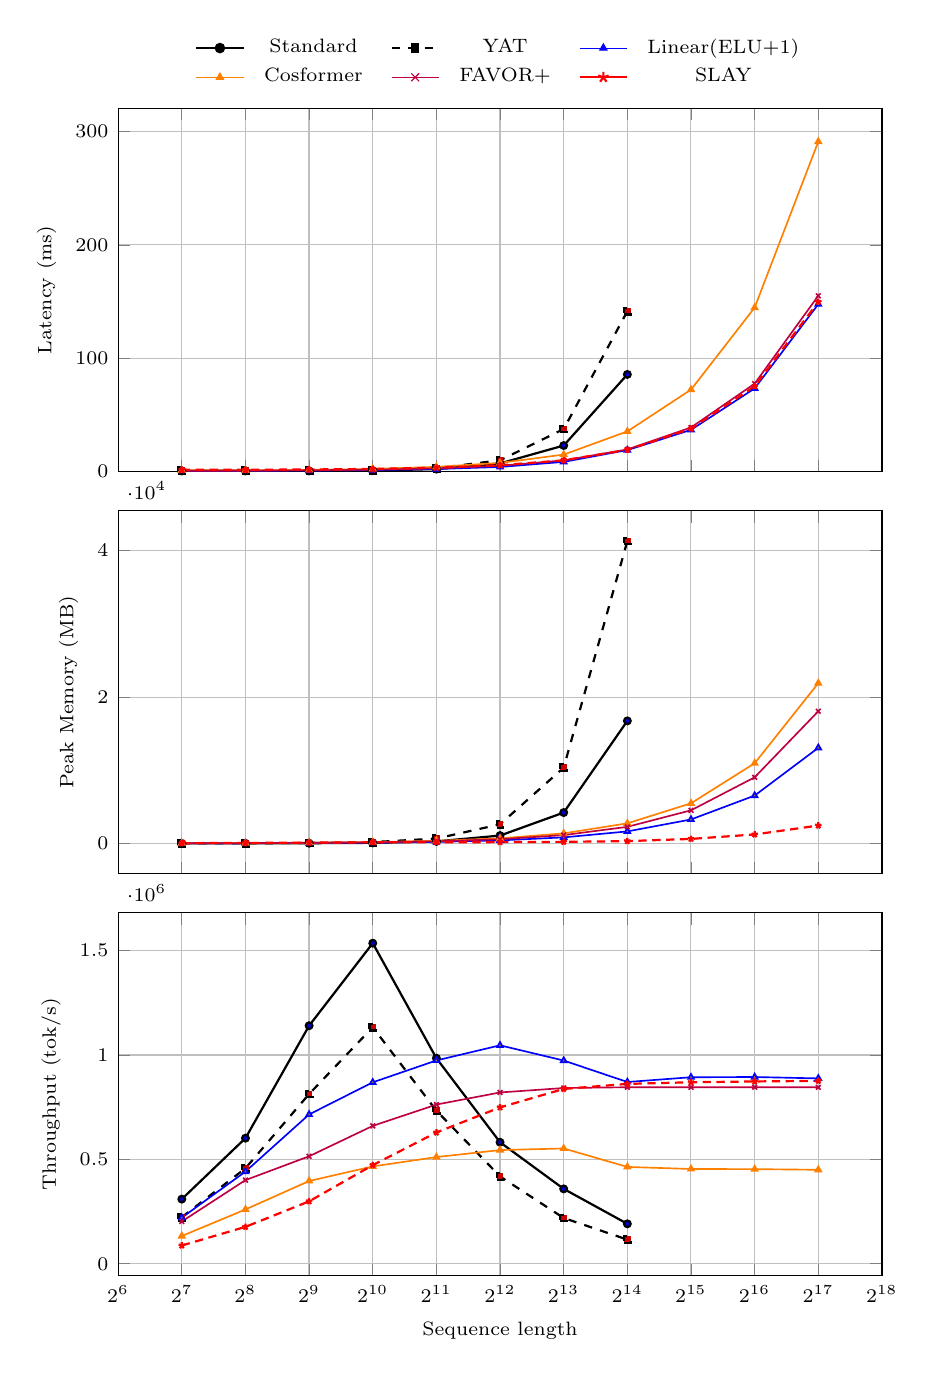
\begin{tikzpicture}

% ================== Legend ==================
\begin{axis}[
    hide axis,
    xmin=0, xmax=1,
    ymin=0, ymax=1,
    width=\columnwidth*.8,
    height=0.38\columnwidth,
    scale only axis,
    legend columns=3,
    legend style={
        font=\scriptsize,
        at={(0.5,1.03)}, 
        anchor=south,
        draw=none,
        column sep=0.5em,
        /tikz/every even column/.append style={column sep=0.8em}
    },
]
\addlegendimage{black, thick, mark=*, mark size=1.5pt}
\addlegendentry{Standard}
\addlegendimage{black, dashed, thick, mark=square*, mark size=1.5pt}
\addlegendentry{YAT}
\addlegendimage{blue, mark=triangle*, mark size=1.5pt}
\addlegendentry{Linear(ELU+1)}
\addlegendimage{orange, mark=triangle*, mark size=1.5pt}
\addlegendentry{Cosformer}
\addlegendimage{purple, mark=x, mark size=2pt}
\addlegendentry{FAVOR+}
\addlegendimage{red, thick, mark=star, mark size=2pt}
\addlegendentry{SLAY}
\end{axis}

% ================== Grouped plots ==================
\begin{groupplot}[
    group style={
        group size=1 by 3,
        vertical sep=0.5cm,
    },
    width=\columnwidth*.8,
    height=0.38\columnwidth,
    xmode=log,
    log basis x=2,
    scale only axis,
    grid=both,
    grid style={line width=0.3pt, gray!30},
    major grid style={line width=0.4pt, gray!50},
    tick label style={font=\scriptsize},
    label style={font=\scriptsize},
    every axis plot/.append style={line width=0.6pt, mark size=1.2pt},
]

% ================== (a) Latency ==================
\nextgroupplot[
    ylabel={Latency (ms)},
    xticklabels={},
    ymin=0,
]

\addplot+[black, thick, mark=*] coordinates {
(128,0.41) (256,0.43) (512,0.45) (1024,0.67)
(2048,2.08) (4096,7.04) (8192,22.84) (16384,85.60)
};
\addplot+[black, dashed, thick, mark=square*] coordinates {
(128,0.57) (256,0.56) (512,0.63) (1024,0.90)
(2048,2.79) (4096,9.79) (8192,37.38) (16384,141.43)
};
\addplot+[blue, mark=triangle*] coordinates {
(128,0.58) (256,0.58) (512,0.72) (1024,1.18)
(2048,2.10) (4096,3.91) (8192,8.42) (16384,18.82)
(32768,36.68) (65536,73.27) (131072,147.63)
};
\addplot+[orange, mark=triangle*] coordinates {
(128,0.96) (256,0.98) (512,1.29) (1024,2.20)
(2048,4.01) (4096,7.52) (8192,14.84) (16384,35.32)
(32768,72.19) (65536,144.60) (131072,291.17)
};
\addplot+[purple, mark=x] coordinates {
(128,0.63) (256,0.64) (512,0.99) (1024,1.55)
(2048,2.69) (4096,4.99) (8192,9.73) (16384,19.38)
(32768,38.77) (65536,77.48) (131072,155.06)
};
\addplot+[red, thick, mark=star] coordinates {
(128,1.46) (256,1.45) (512,1.71) (1024,2.17)
(2048,3.26) (4096,5.47) (8192,9.78) (16384,19.02)
(32768,37.69) (65536,75.05) (131072,149.63)
};

% ================== (b) Memory ==================
\nextgroupplot[
    ylabel={Peak Memory (MB)},
    xticklabels={},
]

\addplot+[black, thick, mark=*] coordinates {
(128,11.9) (256,15.7) (512,29.4) (1024,81.1)
(2048,282.1) (4096,1074.1) (8192,4218.1) (16384,16746.1)
};
\addplot+[black, dashed, thick, mark=square*] coordinates {
(128,13.4) (256,21.7) (512,53.4) (1024,177.2)
(2048,666.3) (4096,2610.4) (8192,10362.6) (16384,41323.1)
};
\addplot+[blue, mark=triangle*] coordinates {
(128,22.9) (256,35.6) (512,61.1) (1024,112.1)
(2048,214.1) (4096,418.1) (8192,826.1) (16384,1642.1)
(32768,3274.1) (65536,6538.1) (131072,13066.1)
};
\addplot+[orange, mark=triangle*] coordinates {
(128,31.5) (256,52.9) (512,95.6) (1024,181.1)
(2048,352.2) (4096,694.2) (8192,1378.2) (16384,2746.3)
(32768,5482.5) (65536,10954.9) (131072,21899.6)
};
\addplot+[purple, mark=x] coordinates {
(128,27.8) (256,45.4) (512,80.7) (1024,151.2)
(2048,292.3) (4096,574.3) (8192,1138.4) (16384,2266.7)
(32768,4523.2) (65536,9036.2) (131072,18062.2)
};
\addplot+[red, thick, mark=star] coordinates {
(128,36.2) (256,62.2) (512,114.2) (1024,151.7)
(2048,160.7) (4096,178.7) (8192,214.7) (16384,314.2)
(32768,618.2) (65536,1226.2) (131072,2442.2)
};

% ================== (c) Throughput ==================
\nextgroupplot[
    ylabel={Throughput (tok/s)},
    xlabel={Sequence length},
]

\addplot+[black, thick, mark=*] coordinates {
(128,309605) (256,601515) (512,1140190) (1024,1535463)
(2048,984540) (4096,581929) (8192,358680) (16384,191393)
};
\addplot+[black, dashed, thick, mark=square*] coordinates {
(128,223026) (256,457217) (512,812948) (1024,1132992)
(2048,733302) (4096,418302) (8192,219174) (16384,115845)
};
\addplot+[blue, mark=triangle*] coordinates {
(128,220935) (256,441509) (512,715210) (1024,869111)
(2048,973777) (4096,1046247) (8192,973413) (16384,870581)
(32768,893397) (65536,894465) (131072,887852)
};
\addplot+[orange, mark=triangle*] coordinates {
(128,132910) (256,260132) (512,396415) (1024,466298)
(2048,511045) (4096,544607) (8192,552194) (16384,463905)
(32768,453914) (65536,453236) (131072,450163)
};
\addplot+[purple, mark=x] coordinates {
(128,202368) (256,400720) (512,514787) (1024,660425)
(2048,762536) (4096,820486) (8192,841800) (16384,845487)
(32768,845161) (65536,845833) (131072,845286)
};
\addplot+[red, thick, mark=star] coordinates {
(128,87397) (256,176813) (512,299006) (1024,472417)
(2048,628732) (4096,748980) (8192,837345) (16384,861529)
(32768,869331) (65536,873279) (131072,875953)
};

\end{groupplot}
\end{tikzpicture}
\end{figure}
% \vspace{-0.5em}

\paragraph{Results overview.}
Figure~\ref{fig:scaling} summarizes the scaling behavior. Quadratic attention mechanisms (standard softmax and exact YAT) exhibit rapidly increasing latency and memory usage, failing beyond \textbf{16K} tokens. In contrast, linear attention methods scale approximately linearly and remain stable up to \textbf{128K} tokens.

SLAY's scaling behavior closely follows and in some cases outperforms other linear attention mechanisms while substantially reducing memory usage relative to its quadratic counterparts. At long sequence lengths, SLAY uses orders of magnitude less memory than exact methods, enabling sequences well beyond where quadratic methods encounter out-of-memory failures. SLAY sustains high throughput comparable to other linear baselines, demonstrating that its added geometric structure does not compromise scalability (see Appendix~\ref{app:scaling-analysis} for detailed comparisons).

\subsection{SLAY on Synthetic Tasks}
\label{subsec:synthetic-experiments}

We evaluate all attention mechanisms on a suite of synthetic sequence modeling tasks
covering basic operations, arithmetic, long-range dependencies, memory, and reasoning. The full results and descriptions of these tasks can be found in the Appendix.

\begin{table}[htbp]
\centering
\small
\caption{Average accuracy by task category. The name of different methods is the same as in Fig. \ref{fig:scaling}.}
\label{tab:summary}

% ---------- Core capabilities ----------
\textbf{(a) Core capabilities}


\makebox[\columnwidth][c]{%
\setlength{\tabcolsep}{3pt}%
\begin{tabular}{lcccc}
\toprule
Method & Basic & Arithmetic & Long-Range & Memory \\
\midrule
Standard        & 0.60 & 0.54 & 0.68 & 0.73 \\
YAT  & 0.52 & 0.53 & 0.68 & 0.73 \\
FAVOR+       & 0.45 & 0.57 & 0.68 & 0.73 \\
Linear          & 0.44 & 0.60 & 0.67 & 0.72 \\
\textbf{SLAY}   & \textbf{0.57} & \textbf{0.57} & \textbf{0.68} & \textbf{0.73} \\
\bottomrule
\end{tabular}%
}

\vspace{0.8em}

% ---------- Higher-level behavior ----------
\textbf{(b) Higher-level behavior}

\makebox[\columnwidth][c]{%
\begin{tabular}{lccc}
\toprule
Method & Patterns & Reasoning & Robustness \\
\midrule
Standard        & 0.83 & 0.56 & 0.80 \\
YAT  & 0.81 & 0.56 & 0.80 \\
FAVOR+       & 0.85 & 0.56 & 0.80 \\
Linear          & 0.85 & 0.56 & 0.80 \\
\textbf{SLAY}   & \textbf{0.86} & \textbf{0.57} & \textbf{0.80} \\
\bottomrule
\end{tabular}%
}

\end{table}

Overall, SLAY matches or exceeds the performance of existing linearized attention mechanisms across the full spectrum of evaluated tasks. As shown in Table~\ref{tab:summary}, SLAY consistently performs on par with the strongest linear baselines on core capabilities such as long‑range dependency modeling and memory, while closing much of the gap to standard attention on basic operations. Notably, SLAY demonstrates competitive or superior accuracy in arithmetic and pattern‑based tasks, and achieves the highest average performance on higher‑level behaviors, including patterns and reasoning. These results indicate that SLAY preserves the representational strengths of linear attention while, in many settings, providing measurable gains over comparable linearized approaches.

\subsection{Extreme Classification Test}
\label{subsec:extreme-classification}
% TODO add results from MM-AmazonTitles-300K LF-AmazonTitles-131K
\textcolor{red}{We have also conducted the extreme classification tests on the Eurlex dataset} and found that the SLAY mechanism provides the best performance across five tested attention methods. Interestingly, it also outperformed
the brute-force softmax attention and regular YAT. The results are summarized in Table \ref{table:extreme_class_tests}.

\begin{table}[htbp]
\centering
\caption{Precision@5 (P@5) results on the Eurlex dataset for different output layer methods.}
\label{tab:eurlex_p5}
\begin{tabular}{l c}
\hline
\textbf{Method} & \textbf{P@5} \\
\hline
Full Softmax      & 0.2638 \\
Performer         & 0.2551 \\
Yat               & 0.2612 \\
Yat (Spherical)   & 0.2597 \\
\textbf{SLAY}     & \textbf{0.2652} \\
\hline
\label{table:extreme_class_tests}
\end{tabular}
\end{table}

% ------------------------------------------------------------
\subsection{\textcolor{red}{SLAYformer: SLAY in Transformers}}
\label{subsec:slayformer}

We now evaluate SLAY in the context of fully trained transformer language models, comparing it against
state‑of‑the‑art linear attention mechanisms and standard softmax attention under identical training
conditions. All models are trained to the same token budget, satisfying the Chinchilla scaling law,
and share architecture, optimization, and data, ensuring a controlled comparison.

Table~\ref{tab:attention-val-comparison} summarizes validation loss and perplexity after training.
Among linear‑time attention mechanisms, SLAY achieves the strongest overall performance, matching or
slightly outperforming FAVOR+ (Performer) and remaining competitive with Cosformer.
Importantly, SLAY does so without introducing additional approximations beyond those already inherent
to linear attention, and without sacrificing stability or convergence speed.

While standard softmax attention remains the strongest performer in absolute terms, its quadratic
computational and memory complexity makes it infeasible at long context lengths.
In contrast, SLAY operates in linear time and memory with respect to sequence length, enabling
scaling to substantially longer contexts while preserving competitive modeling performance.

\begin{table}[htbp]
\centering
\small
\caption{\small{
Validation performance comparison of attention mechanisms after satisfying the Chinchilla scaling law (2.5B tokens processed).
All models are $\sim$125M parameters with context length 1024, embedding dimension 768, 12 layers, 12 attention heads,
trained on FineWeb using learning rate $1\times10^{-4}$ and batch size 32.
Val Loss denotes token‑level cross‑entropy loss on the validation set, and PPL is the corresponding perplexity.
}}
\label{tab:attention-val-comparison}
\resizebox{1\columnwidth}{!}{%
\begin{tabular}{lcc}
\toprule
Method & Val Loss $\downarrow$ & PPL $\downarrow$ \\
\midrule
\textbf{SLAY} & \textbf{5.3463} & \textbf{209.84} \\
FAVOR+ (Performer) & 5.3531 & 211.27 \\
Cosformer & 5.1983 & 180.97 \\
Standard Softmax & 4.6417 & 103.73 \\
\bottomrule
\end{tabular}%
}
\end{table}

Figures~\ref{fig:val-loss-curves} and~\ref{fig:perplexity-curves} provide a detailed view of training
dynamics. Across the full training trajectory, SLAY exhibits stable optimization behavior and
converges at least as quickly as existing linear attention alternatives.
Notably, the gap between SLAY and FAVOR+ steadily narrows over training, and SLAY consistently
matches or exceeds FAVOR+ at convergence in both validation loss and perplexity.
This indicates that the benefits of SLAY are not limited to early‑stage optimization, but persist
through full convergence.

\begin{figure}[htbp]
\centering
\small
\caption{\small{
Validation loss as a function of training steps after satisfying the Chinchilla scaling law.
All models are $\sim$125M parameters, trained on FineWeb with identical optimization settings.
}}
\label{fig:val-loss-curves}
\vspace{0.5em}

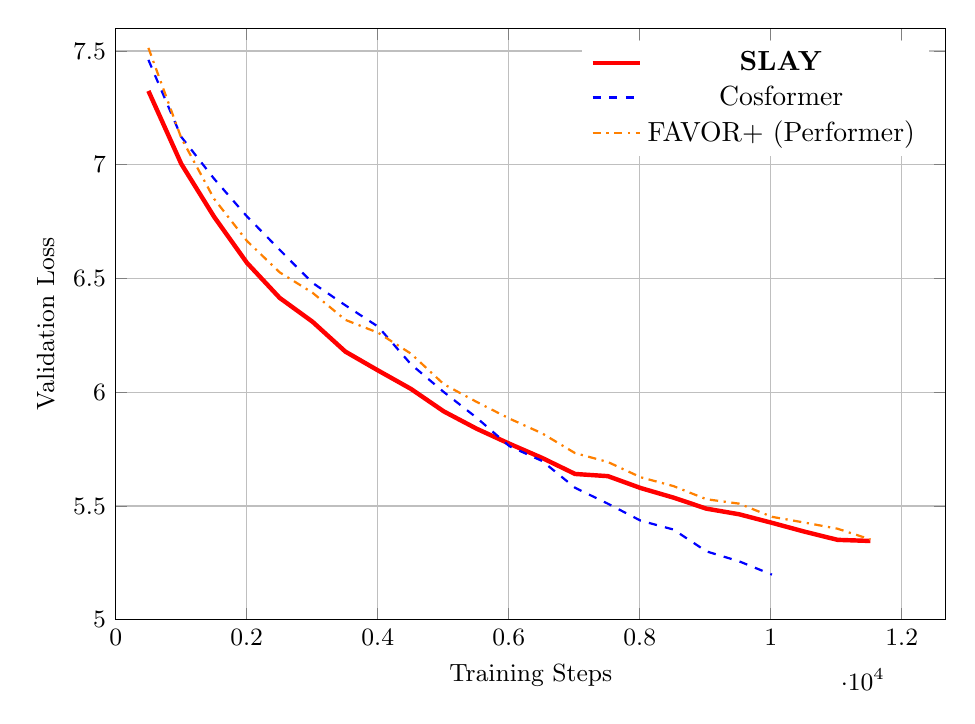
\begin{tikzpicture}
\begin{axis}[
    width=1\columnwidth,
    height=0.75\columnwidth,
    xlabel={Training Steps},
    ylabel={Validation Loss},
    xmin=0,
    ymin=5,
    ymax=7.6,
    grid=both,
    legend style={
        at={(0.98,0.98)},
        anchor=north east,
        draw=none
    },
    tick label style={font=\small},
    label style={font=\small},
]

% ---------- SLAY ----------
\addplot[ultra thick, red]
table[row sep=\\]{
Step Loss\\
500 7.3243\\
1001 7.0039\\
1502 6.7714\\
2003 6.5691\\
2504 6.4146\\
3005 6.3099\\
3506 6.1787\\
4007 6.0955\\
4508 6.0146\\
5009 5.9158\\
5510 5.8397\\
6011 5.7736\\
6512 5.7110\\
7013 5.6408\\
7514 5.6312\\
8015 5.5789\\
8516 5.5368\\
9017 5.4884\\
9518 5.4636\\
10019 5.4260\\
10520 5.3869\\
11021 5.3512\\
11522 5.3463\\
};
\addlegendentry{\textbf{SLAY}}

% ---------- Cosformer ----------
\addplot[thick, dashed, blue]
table[row sep=\\]{
Step Loss\\
500 7.4607\\
1001 7.1226\\
1502 6.9385\\
2003 6.7731\\
2504 6.6259\\
3005 6.4808\\
3506 6.3822\\
4007 6.2881\\
4508 6.1228\\
5009 6.0009\\
5510 5.8881\\
6011 5.7628\\
6512 5.6976\\
7013 5.5801\\
7514 5.5102\\
8015 5.4354\\
8516 5.3964\\
9017 5.3007\\
9518 5.2568\\
10019 5.1983\\
};
\addlegendentry{Cosformer}

% ---------- FAVOR+ (Performer) ----------
\addplot[thick, dash dot, orange]
table[row sep=\\]{
Step Loss\\
500 7.5135\\
1001 7.1177\\
1502 6.8503\\
2003 6.6652\\
2504 6.5269\\
3005 6.4373\\
3506 6.3182\\
4007 6.2614\\
4508 6.1696\\
5009 6.0353\\
5510 5.9576\\
6011 5.8842\\
6512 5.8190\\
7013 5.7325\\
7514 5.6934\\
8015 5.6263\\
8516 5.5874\\
9017 5.5298\\
9518 5.5103\\
10019 5.4524\\
10520 5.4269\\
11021 5.4001\\
11522 5.3531\\
};
\addlegendentry{FAVOR+ (Performer)}

\end{axis}
\end{tikzpicture}
\end{figure}

\begin{figure}[htbp]
\centering
\small
\caption{\small{
Validation perplexity as a function of training steps after satisfying the Chinchilla scaling law.
All models are $\sim$125M parameters, trained on FineWeb with identical optimization settings.
}}
\label{fig:perplexity-curves}
\vspace{0.5em}

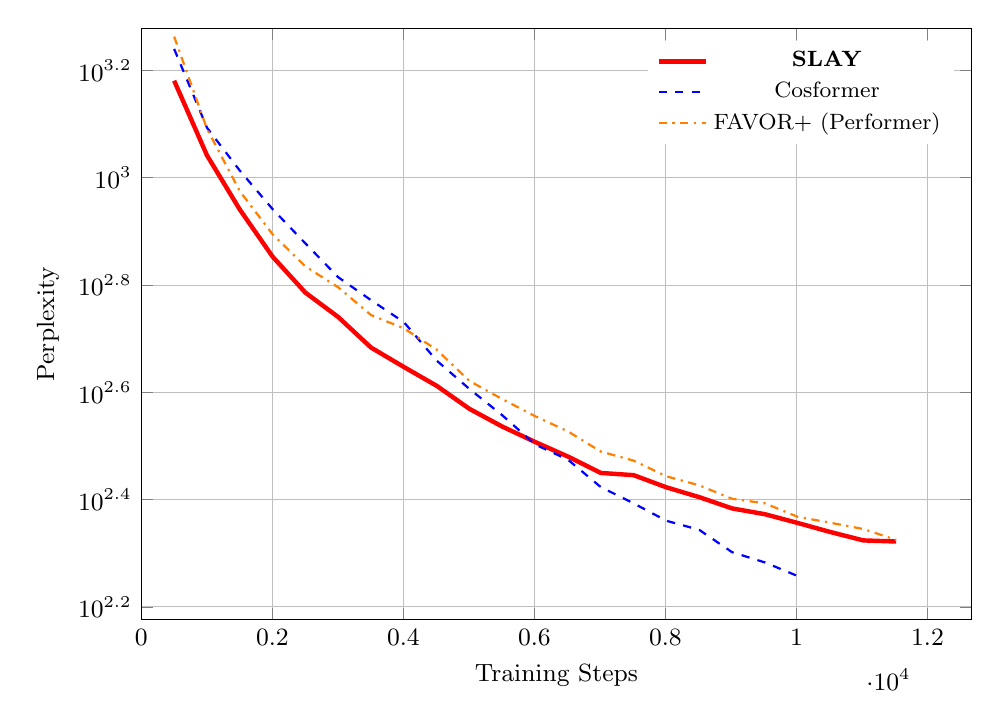
\begin{tikzpicture}
\begin{axis}[
    width=1\columnwidth,
    height=0.75\columnwidth,
    xlabel={Training Steps},
    ylabel={Perplexity},
    xmin=0,
    ymin=150,
    ymax=1900,
    ymode=log,
    grid=both,
    legend style={
        at={(0.98,0.98)},
        anchor=north east,
        draw=none,
        font=\footnotesize
    },
    tick label style={font=\small},
    label style={font=\small},
]

% ---------- SLAY ----------
\addplot[ultra thick, red]
table[row sep=\\]{
Step PPL\\
500 1516.78\\
1001 1100.96\\
1502 872.50\\
2003 712.69\\
2504 610.68\\
3005 549.98\\
3506 482.37\\
4007 443.86\\
4508 409.38\\
5009 370.83\\
5510 343.67\\
6011 321.70\\
6512 302.17\\
7013 281.67\\
7514 279.00\\
8015 264.78\\
8516 253.87\\
9017 241.88\\
9518 235.94\\
10019 227.24\\
10520 218.53\\
11021 210.86\\
11522 209.84\\
};
\addlegendentry{\textbf{SLAY}}

% ---------- Cosformer ----------
\addplot[thick, dashed, blue]
table[row sep=\\]{
Step PPL\\
500 1738.36\\
1001 1239.66\\
1502 1031.22\\
2003 873.99\\
2504 754.40\\
3005 652.48\\
3506 591.22\\
4007 538.14\\
4508 456.14\\
5009 403.79\\
5510 360.73\\
6011 318.25\\
6512 298.14\\
7013 265.10\\
7514 247.19\\
8015 229.39\\
8516 220.60\\
9017 200.48\\
9518 191.86\\
10019 180.97\\
};
\addlegendentry{Cosformer}

% ---------- FAVOR+ (Performer) ----------
\addplot[thick, dash dot, orange]
table[row sep=\\]{
Step PPL\\
500 1832.56\\
1001 1233.66\\
1502 944.18\\
2003 784.63\\
2504 683.26\\
3005 624.74\\
3506 554.59\\
4007 523.95\\
4508 477.98\\
5009 417.93\\
5510 386.70\\
6011 359.30\\
6512 336.64\\
7013 308.74\\
7514 296.90\\
8015 277.64\\
8516 267.04\\
9017 252.10\\
9518 247.24\\
10019 233.32\\
10520 227.44\\
11021 221.42\\
11522 211.27\\
};
\addlegendentry{FAVOR+ (Performer)}

\end{axis}
\end{tikzpicture}
\end{figure}

Taken together, these results demonstrate that SLAY is at least as effective as state‑of‑the‑art
linear-time attention mechanisms in practical transformer training.
This finding is particularly significant in light of the theoretical properties of the YAT kernel
introduced in Section ~\ref{sec:intro}.
By enabling an efficient linear‑attention implementation of YAT, SLAY makes it possible to train
large‑scale transformer models (SLAYformers) with long input sequences while preserving the kernel’s desirable
theoretical properties, without incurring the prohibitive quadratic cost and without sacrificing core modeling performance relative to existing linear alternatives.

As a result, SLAY provides a practical path toward scalable long‑context transformers that combine
strong empirical performance with scalable, geometry-aware kernels, positioning it as a compelling drop‑in
replacement for existing linear attention mechanisms in large‑scale settings.

% ------------------------------------------------------------
% 9. Conclusion
% ------------------------------------------------------------
\section{Conclusion}
\label{sec:conclusion}

We introduced SLAY: Spherical Linearized Attention with YAT-Kernel, a linear-time attention mechanism that makes the \E-product operator from Neural Matter Networks (NMNs) practical for long-context sequence modeling. By enforcing unit-norm constraints, applying Bernstein’s Theorem, and approximating the resulting kernel with strictly positive Tensor Product Random Features, we obtain a factorizable and bounded attention kernel compatible with previous low-rank factorized attention techniques, extensively used before \citep{performers}.

Theoretical analysis shows that the proposed approximation preserves the self-regulation and superposition properties of the original \E-product. Empirically, we demonstrate stable end-to-end training, linear time and memory scaling, and the ability to process sequences \textbf{30x} longer than those handled by standard attention mechanism on a single 80 GB GPU.

Taken together, these results suggest that the SLAY mechanism \textit{(spherical linearized attention with Yat Kernel)} offers a viable path toward scalable, geometry-aware attention mechanisms, bridging NMNs and practical long-context Transformers. More broadly, this work also demonstrates that attention mechanisms need not be restricted to softmax-like similarities to admit linear-time computation. By combining spherical geometry with general kernel linearization tools, Spherical Yat-Attention opens a path toward scalable attention mechanisms grounded in alternative interaction principles.

\section*{Impact Statement}
This paper presents work whose goal is to advance the field of Machine Learning. There are
many potential societal consequences of our work, none which we feel must be specifically highlighted here. We would like to note though that linear attention Transformer models, that \textbf{SLAY} can power, address the challenge of the large carbon footprint in training of their brute force and much more computationally intense counterparts. In addition, we believe that scalable geometry-aware mechanisms like SLAY will pave the way for lighter, safer and more interpretable models. We have made every effort to ensure the work’s reproducibility, in particular by providing details regarding hyperparameter settings and direct access to a code respository in the Appendix. 
% ============================================================
% References
% ============================================================
\bibliography{references}
\bibliographystyle{icml2026}


%\begin{thebibliography}{9}




\clearpage
\onecolumn

\section*{Appendix}
\appendix
\section{Background Results}
\label{app:background}

This section collects standard background facts used in the main text.

\begin{adjustwidth}{1.5em}{1.5em}
\begin{lemma}[Bernstein Representation Applicability]
\label{lem:complete-monotone}
For $\epsilon > 0$ and $C = 2 + \epsilon$, the variable $y = C - 2x$ satisfies $y \geq \epsilon > 0$ for all $x \in [-1,1]$. Hence Bernstein's representation $1/(C - 2x) = \int_0^\infty e^{-s(C-2x)}\,ds$ applies throughout the domain.
\end{lemma}
\begin{proof}
See Appendix~\ref{app:additional-proofs}.
\end{proof}
\end{adjustwidth}

\section{Geometric Interpretation and Invariances}
\label{app:geom}

This appendix expands on the geometric view of the spherical \E-product discussed in Section~\ref{sec:method}. On $\Sph^{d-1}$, the squared chordal distance satisfies
$d_{\Sph^{d-1}}(\widehat{\mathbf{q}},\widehat{\mathbf{k}})^2
= 2\bigl(1-\widehat{\mathbf{q}}^\top \widehat{\mathbf{k}}\bigr)$,
so the spherical kernel can be interpreted as an $\epsilon$-regularized chordal-distance interaction.

\begin{adjustwidth}{1.5em}{1.5em}
\begin{proposition}[Geometric Origin]
\label{prop:geometric}
The spherical \E-product is an $\epsilon$-regularized chordal-distance interaction on $\Sph^{d-1}$:
\[
\E_{\mathrm{sph}}(\widehat{\mathbf{q}}, \widehat{\mathbf{k}})
=
\frac{\langle \widehat{\mathbf{q}}, \widehat{\mathbf{k}} \rangle^2}
     {d_{\Sph^{d-1}}(\widehat{\mathbf{q}}, \widehat{\mathbf{k}})^2 + \epsilon},
\]
where the numerator captures directional alignment and the denominator enforces locality via chordal proximity.
\end{proposition}
\end{adjustwidth}

Since the kernel depends only on
$\widehat{\mathbf{q}}^\top \widehat{\mathbf{k}}$,
it belongs to the class of isotropic kernels on the sphere.
All spherical positive-definiteness claims in the main text assume $d\ge 2$,
where Schoenberg's characterization applies \citep{schoenberg1942}.

\begin{adjustwidth}{1.5em}{1.5em}
\begin{remark}[Geometric Invariances]
\label{rem:invariances}
The spherical $\E$-product is invariant under
(i) rotations:
$\E_{\mathrm{sph}}(\mathbf{R}\widehat{\mathbf{q}}, \mathbf{R}\widehat{\mathbf{k}})
= \E_{\mathrm{sph}}(\widehat{\mathbf{q}}, \widehat{\mathbf{k}})$
for all $\mathbf{R} \in SO(d)$,
and (ii) uniform scaling prior to normalization.
Note that while
$(\widehat{\mathbf{q}}^\top \widehat{\mathbf{k}})^2$
is even under sign flips, the full kernel
\[
\E_{\mathrm{sph}}(\widehat{\mathbf{q}},\widehat{\mathbf{k}})
=
\frac{(\widehat{\mathbf{q}}^\top \widehat{\mathbf{k}})^2}
     {(2+\epsilon)-2\widehat{\mathbf{q}}^\top\widehat{\mathbf{k}}}
\]
is not invariant under $\widehat{\mathbf{q}} \mapsto -\widehat{\mathbf{q}}$
in general.
\end{remark}
\end{adjustwidth}

\begin{adjustwidth}{1.5em}{1.5em}
\begin{proposition}[PRF Unbiasedness]
\label{prop:prf-unbiased}
For $\widehat{\mathbf{q}}, \widehat{\mathbf{k}} \in \Sph^{d-1}$ and
$\{\boldsymbol{\omega}_i\}_{i=1}^D
\stackrel{\mathrm{iid}}{\sim} \mathcal{N}(\mathbf{0}, \mathbf{I}_d)$:
\[
\mathbb{E}\!\left[
\left\langle
\phi_{\text{PRF}}(\widehat{\mathbf{q}}; s),
\phi_{\text{PRF}}(\widehat{\mathbf{k}}; s)
\right\rangle
\right]
=
e^{2s\,\widehat{\mathbf{q}}^\top \widehat{\mathbf{k}}}.
\]
\end{proposition}
\begin{proof}
See Appendix~\ref{app:additional-proofs}.
\end{proof}
\end{adjustwidth}

\begin{adjustwidth}{1.5em}{1.5em}
\begin{lemma}[Positive Mixture Closure]
\label{lem:mixture-pd}
If $\{k_s\}_{s \geq 0}$ is a family of positive-definite kernels on $\mathcal{X}$
and $w(s) \geq 0$ is a nonnegative measure, then
$k(x,y) = \int_0^\infty w(s)\,k_s(x,y)\,ds$
is PD on $\mathcal{X}$ (a standard closure property of PD kernels;
see, e.g., \citep{aronszajn1950,scholkopf2002learning}).
\end{lemma}
\end{adjustwidth}

\begin{adjustwidth}{1.5em}{1.5em}
\begin{theorem}[Tensor Kernel Decomposition]
\label{thm:tensor-rkhs}
Let $k_1, k_2$ be positive-definite kernels on $\mathcal{X}$
with RKHSs $\mathcal{H}_1, \mathcal{H}_2$.
Then the product kernel
$k(x,y) = k_1(x,y) \cdot k_2(x,y)$
is positive definite with RKHS
$\mathcal{H} = \mathcal{H}_1 \otimes \mathcal{H}_2$
(see, e.g., \citep{aronszajn1950,berlinet2004}).
\end{theorem}
\end{adjustwidth}

\section{Preliminaries: Polynomial Kernel Approximations}
\label{app:prelim-poly}

We summarize three approximations of the degree-2 polynomial kernel
$k_{\text{poly}}(x,y)=(x^\top y)^2$ used in our implementation and ablations.
Let $x,y\in\R^d$.

\paragraph{Random Maclaurin (RM).}
Draw Rademacher vectors $r_i, s_i\in\{\pm1\}^d$ and define
\[
\phi_{\text{RM}}(x)=\frac{1}{\sqrt{P}}\bigl[(r_i^\top x)(s_i^\top x)\bigr]_{i=1}^P.
\]
Then $\mathbb{E}[\langle \phi_{\text{RM}}(x),\phi_{\text{RM}}(y)\rangle]=(x^\top y)^2$ \citep{karkarnick2012}.
RM is unbiased but can have high variance for small $P$.

\paragraph{Nystrom features.}
Let anchors $A=\{a_1,\dots,a_P\}\subset\R^d$ and define
$K_{AA}\in\R^{P\times P}$ with $(K_{AA})_{ij}=(a_i^\top a_j)^2$.
Given $K_{AA}+\lambda I$, define
\[
\phi_{\text{Nys}}(x)=(K_{xA})(K_{AA}+\lambda I)^{-1/2},\quad K_{xA}=[(x^\top a_i)^2]_{i=1}^P.
\]
This yields a low-rank approximation whose quality depends on anchor coverage and conditioning \citep{williams2001nystrom}.

\paragraph{Anchor (low-rank) features.}
Using the same anchors $A$, define
\[
\phi_{\text{Anc}}(x)=\frac{1}{\sqrt{P}}\bigl[(x^\top a_i)^2\bigr]_{i=1}^P.
\]
This is a simple low-rank approximation; it is not unbiased in general but is often stable for small $P$.

\paragraph{Comparison.}
RM is unbiased but variance-dominated at small feature budgets; Nystrom reduces variance if anchors are well-conditioned; anchor features are computationally simplest and empirically most stable at small $P$.

\section{Ablation: Polynomial Approximation Sweep}
\label{app:poly-ablation}

This appendix reports the multi-scale kernel-fidelity sweep referenced in Section~\ref{subsec:poly-ablation}. All variants tie the $\mathrm{QKV}$ and output projection weights and compare outputs against exact kernel-normalized spherical \E-attention.

\begin{table}[t]
\centering
\small
\caption{Multi-scale ablation over feature budgets for polynomial-kernel approximations. We compare attention outputs against \emph{exact kernel-normalized} spherical YAT with tied QKV/out projections. Lower Rel.~$\ell_2$ is better; latency is forward-pass time.}
\label{tab:poly-sweep}
\begin{tabular}{llcccccc}
\toprule
Scale & Method & $T$ & $R$ & $M$ & $P$ & Rel.~$\ell_2\downarrow$ & Latency (ms)$\downarrow$\\
\midrule
Small & Exact (Spherical) & 128 & 2 & 8 & 8 & 0.0000 & 3.12\\
 & Laplace-only &  &  &  &  & 0.5870 & 2.78\\
 & Anchor &  &  &  &  & 0.6626 & 3.82\\
 & Hadamard (shared $\omega$) &  &  &  &  & 0.8237 & 3.34\\
 & Nystrom &  &  &  &  & 22.9072 & 3.41\\
 & TensorSketch &  &  &  &  & 474075.1562 & 5.17\\
 & Random Maclaurin &  &  &  &  & 2195912.7500 & 5.59\\
\addlinespace
Medium & Exact (Spherical) & 256 & 2 & 16 & 16 & 0.0000 & 0.79\\
 & Laplace-only &  &  &  &  & 0.5417 & 16.10\\
 & Anchor &  &  &  &  & 0.5667 & 18.54\\
 & Hadamard (shared $\omega$) &  &  &  &  & 0.6609 & 17.44\\
 & Nystrom &  &  &  &  & 61.6529 & 18.46\\
 & TensorSketch &  &  &  &  & 214115.9844 & 19.01\\
 & Random Maclaurin &  &  &  &  & 1715766.8750 & 18.80\\
\addlinespace
Large & Exact (Spherical) & 512 & 2 & 32 & 32 & 0.0000 & 5.02\\
 & Laplace-only &  &  &  &  & 0.4850 & 1905.80\\
 & Anchor &  &  &  &  & 0.4939 & 489.42\\
 & Hadamard (shared $\omega$) &  &  &  &  & 0.6793 & 1932.07\\
 & Nystrom &  &  &  &  & 28.1970 & 569.64\\
 & TensorSketch &  &  &  &  & 461739.0312 & 547.76\\
 & Random Maclaurin &  &  &  &  & 1772757.5000 & 551.43\\
\addlinespace
\bottomrule
\end{tabular}
\end{table}
\section{Integral Representation of the Spherical \E-Product}
\label{app:integral}

In this appendix, we provide a detailed derivation of the integral representation used to linearize the spherical \E-product kernel.

Recall that under the unit-norm constraint $\hat q, \hat k \in \Sph^{d-1}$, the \E-product reduces to
\begin{equation}
\E_{\mathrm{sph}}(\hat q, \hat k)
= \frac{x^2}{C - 2x},
\qquad
x = \hat q^\top \hat k \in [-1,1],
\quad
C = 2 + \epsilon.
\label{eq:app-spherical}
\end{equation}

The function $g(y) = 1/y$ is completely monotone on $(0,\infty)$ and therefore admits the Bernstein representation
\begin{equation}
\frac{1}{y} = \int_0^\infty e^{-s y}\, ds.
\label{eq:app-bernstein}
\end{equation}

Applying this identity with $y = C - 2x$, we obtain
\begin{align}
\E_{\mathrm{sph}}(\hat q, \hat k)
&= x^2 \int_0^\infty e^{-s(C - 2x)} \, ds \\
&= \int_0^\infty e^{-sC} \, x^2 e^{2s x} \, ds.
\label{eq:app-integral}
\end{align}

This representation expresses the spherical \E-product as a positively weighted mixture of a degree-2 polynomial kernel and an exponential kernel in the angular variable $x$. This decomposition forms the basis for the random-feature approximation introduced in the main text.

\section{Random Feature Construction and Unbiasedness}
\label{app:features}

In this appendix, we provide additional details on the random-feature construction used to approximate the integrand appearing in the spherical \E-product representation and justify its unbiasedness.

Recall from Eq.~\eqref{eq:integral} that the spherical \E-product admits the decomposition
\[
\E_{\mathrm{sph}}(\hat q, \hat k)
= \int_0^\infty e^{-sC} \, x^2 e^{2s x} \, ds,
\qquad x = \hat q^\top \hat k.
\]

\paragraph{Polynomial component.}
The term $x^2 = (\hat q^\top \hat k)^2$ corresponds to a homogeneous degree-2 polynomial kernel. This kernel admits an explicit feature map given by
\[
\phi_{\mathrm{poly}}(u) = \mathrm{vec}(u u^\top),
\]
or an approximate variant implemented via tensor sketching. In both cases, the inner product of feature maps yields an unbiased estimator of the polynomial kernel.

\paragraph{Exponential component.}
The exponential term $e^{2s x}$ is approximated using strictly positive random features. For random projections $\omega$ drawn from a Gaussian or orthogonal distribution, the feature map
\[
\phi_{\mathrm{PRF}}(u; s)
=
\frac{1}{\sqrt{D}}\exp\!\left(\sqrt{2s}\,\omega^\top u - s\right)
\]
satisfies
\[
\mathbb{E}\big[ \langle \phi_{\mathrm{PRF}}(\hat q; s), \phi_{\mathrm{PRF}}(\hat k; s) \rangle \big]
= e^{2s\, \hat q^\top \hat k}.
\]

\paragraph{Tensor product approximation.}
Since the polynomial component can be computed exactly (or approximated in practice) and the exponential component is estimated with unbiased PRFs, their tensor product
\[
\phi_{\mathrm{poly}}(u) \otimes \phi_{\mathrm{PRF}}(u; s)
\]
is an unbiased estimator of the product kernel $x^2 e^{2s x}$ by linearity of expectation. Approximating the outer integral using quadrature preserves unbiasedness up to the discretization error introduced by the numerical integration scheme.

\paragraph{On ``pure Laplace'' forms.}
If one insists on a nonnegative Laplace mixture of plain exponentials $e^{2sx}$, then $x^2/(C-2x)$ cannot be represented exactly, because $k(0)=0$ whereas $\int_0^\infty w(s)\,e^{2s\cdot 0}\,ds=\int_0^\infty w(s)\,ds\ge 0$ for any $w\ge 0$.
There is, however, an exact decomposition that removes the explicit $x^2$ factor at the cost of an affine correction term:
\[
\frac{x^2}{C-2x}
=
\frac{C^2}{4}\int_0^\infty e^{-Cs}\,e^{2sx}\,ds\; -\;\frac{C}{4}\; -\;\frac{x}{2}.
\]
This identity follows from $x^2 e^{2sx}=\tfrac{1}{4}\,\partial_s^2 e^{2sx}$ and two integrations by parts, whose boundary terms yield the affine correction.
While this removes the need for polynomial random features, it introduces signed components (through the subtraction of constant and linear kernels) and therefore does not retain the ``strictly positive feature map'' and denominator-positivity guarantees emphasized in the main construction.

\paragraph{Hadamard (elementwise) fusion variant.}
Some implementations replace the tensor product with elementwise (Hadamard) fusion,
\[\phi_{\mathrm{had}}(u; s)=\sqrt{w_r}\,\bigl(\phi_{\mathrm{poly}}(u)\odot \phi_{\mathrm{PRF}}(u; s)\bigr),\]
which yields a valid positive feature map but targets a \emph{different} kernel than the tensor product. In particular, the expected inner product becomes
\[\mathbb{E}[\langle \phi_{\mathrm{had}}(\hat q; s),\phi_{\mathrm{had}}(\hat k; s)\rangle]\;\approx\;(\hat q^\top \hat k)^2\,e^{2s\,\hat q^\top \hat k}\quad\text{only if }\phi_{\mathrm{poly}}\text{ and }\phi_{\mathrm{PRF}}\text{ are aligned feature maps.}\]
With standard independent random features, Hadamard fusion instead corresponds to a product of marginal kernels across matched feature indices, which generally introduces bias relative to the target integrand kernel. The benefit is computational: it avoids the $D_p\times D_r$ tensor expansion and reduces memory, but at the cost of a kernel mismatch. We therefore treat Hadamard fusion as a fast baseline rather than the primary estimator of the spherical \E-product.

\section{Positivity and Stability Guarantees}
\label{app:stability}

This appendix provides additional justification for the positivity and numerical stability properties of the proposed linearized \E-attention mechanism.

\paragraph{Positivity.}
All components of the \emph{target} spherical kernel are non-negative. Moreover, if the polynomial feature map is computed exactly (or with a positivity-preserving approximation), then the corresponding approximate scores are non-negative:
\begin{itemize}[leftmargin=1.4em]
    \item The polynomial term $(\hat q^\top \hat k)^2$ is non-negative for all $\hat q, \hat k \in \Sph^{d-1}$.
    \item The exponential term $e^{2s x}$ is strictly positive for all $s \ge 0$ and $x \in [-1,1]$.
    \item The quadrature weights $w_r$ are non-negative.
\end{itemize}
Consequently, under this condition the approximate attention scores produced by the tensor-product random features are non-negative.

\paragraph{Numerical stability.}
The boundedness of the spherical \E-product on $\Sph^{d-1}$ (Proposition~\ref{prop:bounded}) implies that attention scores remain uniformly bounded. Combined with positivity, this prevents the numerical instabilities associated with oscillatory random features and negative attention weights. This behavior mirrors stability properties previously observed in positive random
feature–based linear attention mechanisms \citep{performers}.

\section{Experimental and Implementation Details}
\label{app:experiments}

This appendix summarizes additional experimental and implementation details to facilitate reproducibility.

\paragraph{Random feature configuration.}
Unless otherwise stated, all experiments use a fixed number of random features per attention head. Quadrature nodes and weights are chosen using standard numerical integration schemes and shared across heads and layers.

\paragraph{Normalization.}
Queries and keys are explicitly normalized to unit norm prior to feature computation. This normalization is applied per attention head and does not introduce additional learnable parameters.

\paragraph{Hardware and software.}
All experiments were conducted using PyTorch on NVIDIA A100 GPUs with ~80\,GB of memory. Attention-only benchmarks use custom linear-attention operators, while full-model experiments rely on standard PyTorch modules augmented with the proposed attention mechanism.

\paragraph{Training configuration.}
Optimizer settings, learning rates, batch sizes, and training schedules are kept identical across softmax and \E-based attention variants unless otherwise specified. This ensures that observed differences are attributable to the attention mechanism rather than auxiliary training effects.

\paragraph{Ablation protocol (polynomial approximations).}
The kernel-fidelity ablation in Section~\ref{subsec:poly-ablation} is implemented in \texttt{tests/ablation\_poly\_approx.py}. Running the script with \texttt{--sweep} produces a LaTeX table in \texttt{tables/poly\_ablation\_sweep.tex}. All variants tie the $\mathrm{QKV}$ and output projection weights and compare outputs against exact kernel-normalized spherical \E-attention.

\paragraph{Detailed Synthetic Test Results.}

Below is a summary of the categories of and specific synthetic tests ran. 

\begin{table}[htbp]
\centering
\small
\caption{\small{
Overview of benchmark task categories used in our evaluation.
Each category groups tasks designed to probe specific capabilities of sequence models.
See \texttt{docs/BENCHMARK\_TASKS.md} in the project code repository for detailed task descriptions.
}}
\label{tab:task-categories}
\resizebox{1\columnwidth}{!}{%
\begin{tabular}{lll}
\toprule
\textbf{Category} & \textbf{Tasks} & \textbf{Tests} \\
\midrule
Basic &
copy, sort, reverse &
Information routing \\

Memory &
retrieval, kv\_recall, first\_token, selective\_copy &
Sparse retrieval, associative memory \\

Long-Range &
long\_copy, distant\_match, multihop &
Long-range dependencies \\

Reasoning &
stack, induction, pattern &
State tracking, pattern matching \\

Arithmetic &
counting, parity, addition, modular &
Aggregation \\

Pattern &
bigram, majority &
Statistical patterns \\

Robustness &
noisy\_copy, compression &
Noise filtering \\

Aggregation &
histogram &
Multi-class counting \\
\bottomrule
\end{tabular}%
}
\end{table}

Below (Table \ref{tab:tasks-all}) provides a fully detailed results of said synthetic tests.

\setlength{\textfloatsep}{8pt}
\vspace{-0.5em}
\begin{table}[!htbp]
\centering
\small
\caption{Synthetic task performance across all categories. Accuracy (mean $\pm$ std over 3 seeds).}
\label{tab:tasks-all}
\begin{tabular}{lccccc}
\toprule
Task & Standard & Spherical--YAT & Performer & Linear & SLAY \\
\midrule
\multicolumn{6}{l}{\emph{Basic}} \\
Copy            & 1.00$\pm$0.00 & 1.00$\pm$0.00 & 1.00$\pm$0.00 & 1.00$\pm$0.00 & 1.00$\pm$0.00 \\
Sort            & 0.28$\pm$0.02 & 0.24$\pm$0.01 & 0.27$\pm$0.02 & 0.26$\pm$0.02 & 0.29$\pm$0.01 \\
Reverse         & 0.51$\pm$0.00 & 0.33$\pm$0.02 & 0.09$\pm$0.01 & 0.05$\pm$0.01 & 0.42$\pm$0.04 \\
\midrule
\multicolumn{6}{l}{\emph{Arithmetic}} \\
Counting        & 0.72$\pm$0.01 & 0.78$\pm$0.04 & 0.81$\pm$0.06 & 0.83$\pm$0.05 & 0.74$\pm$0.13 \\
Parity          & 0.49$\pm$0.03 & 0.49$\pm$0.03 & 0.49$\pm$0.03 & 0.49$\pm$0.03 & 0.49$\pm$0.03 \\
Addition        & 0.78$\pm$0.03 & 0.68$\pm$0.16 & 0.84$\pm$0.02 & 0.91$\pm$0.04 & 0.86$\pm$0.05 \\
Modular         & 0.15$\pm$0.03 & 0.16$\pm$0.01 & 0.15$\pm$0.02 & 0.15$\pm$0.03 & 0.20$\pm$0.03 \\
\midrule
\multicolumn{6}{l}{\emph{Long-Range}} \\
Long Copy       & 1.00$\pm$0.00 & 1.00$\pm$0.00 & 1.00$\pm$0.00 & 1.00$\pm$0.00 & 1.00$\pm$0.00 \\
Distant Match   & 1.00$\pm$0.00 & 1.00$\pm$0.00 & 1.00$\pm$0.00 & 0.99$\pm$0.02 & 1.00$\pm$0.00 \\
Multihop        & 0.04$\pm$0.01 & 0.04$\pm$0.01 & 0.03$\pm$0.02 & 0.03$\pm$0.00 & 0.04$\pm$0.01 \\
\midrule
\multicolumn{6}{l}{\emph{Memory}} \\
Retrieval       & 1.00$\pm$0.00 & 1.00$\pm$0.00 & 1.00$\pm$0.00 & 1.00$\pm$0.00 & 1.00$\pm$0.00 \\
Kv Recall       & 0.02$\pm$0.02 & 0.02$\pm$0.03 & 0.03$\pm$0.00 & 0.02$\pm$0.02 & 0.02$\pm$0.01 \\
First Token     & 1.00$\pm$0.00 & 1.00$\pm$0.00 & 1.00$\pm$0.00 & 0.97$\pm$0.02 & 1.00$\pm$0.00 \\
Selective Copy  & 0.88$\pm$0.00 & 0.88$\pm$0.00 & 0.88$\pm$0.00 & 0.88$\pm$0.00 & 0.88$\pm$0.00 \\
\midrule
\multicolumn{6}{l}{\emph{Patterns}} \\
Bigram          & -- & -- & -- & -- & -- \\
Majority        & 0.78$\pm$0.07 & 0.75$\pm$0.06 & 0.82$\pm$0.02 & 0.82$\pm$0.06 & 0.84$\pm$0.03 \\
Histogram       & 0.87$\pm$0.00 & 0.87$\pm$0.00 & 0.87$\pm$0.00 & 0.87$\pm$0.00 & 0.87$\pm$0.00 \\
\midrule
\multicolumn{6}{l}{\emph{Reasoning}} \\
Stack           & 0.75$\pm$0.01 & 0.75$\pm$0.01 & 0.76$\pm$0.01 & 0.75$\pm$0.01 & 0.76$\pm$0.01 \\
Induction       & 0.02$\pm$0.02 & 0.02$\pm$0.02 & 0.02$\pm$0.01 & 0.01$\pm$0.01 & 0.03$\pm$0.01 \\
Pattern         & 0.91$\pm$0.00 & 0.91$\pm$0.00 & 0.91$\pm$0.00 & 0.91$\pm$0.00 & 0.91$\pm$0.00 \\
\midrule
\multicolumn{6}{l}{\emph{Robustness}} \\
Noisy Copy      & 1.00$\pm$0.00 & 1.00$\pm$0.00 & 1.00$\pm$0.00 & 1.00$\pm$0.00 & 1.00$\pm$0.00 \\
Compression     & 0.59$\pm$0.00 & 0.59$\pm$0.00 & 0.59$\pm$0.01 & 0.59$\pm$0.01 & 0.59$\pm$0.01 \\
\bottomrule
\end{tabular}
\end{table}
\vspace{-0.5em}

\paragraph{Code availability.}
An open-source implementation of the SLAY mechanism, including training scripts and experimental configurations, is available at
\url{https://anonymous.4open.science/r/slay-3B7C}.


\section{Implementation Notes: Quadrature Scaling and Shapes}
\label{app:impl}

\paragraph{Practical knobs and defaults.}
In our implementation, $R$ controls the quadrature accuracy of the Laplace integral and $D$ controls the Monte Carlo variance of PRF. The polynomial approximation uses either a feature dimension $D_p$ (e.g., Random Maclaurin or TensorSketch) or an anchor count $P$ (anchor features or Nystrom); by default we use anchor features because they preserve non-negativity of the polynomial component and are stable at small budgets.
The tensor-product fusion uses a sketch dimension $D_t$, trading accuracy for compute/memory. We use small stabilizers $\epsilon$ (kernel) and $\delta$ (attention denominator) for numerical robustness.

\paragraph{Remark (explicit tensor product).}
Without sketching, the per-node tensor-product feature dimension is $D_pD$ and the resulting attention cost would scale as $O(L\,R\,D_pD)$ rather than $O(L\,R\,D_t)$. We use sketching to avoid explicitly materializing Kronecker vectors while preserving the same target product-kernel structure up to controlled approximation error.

\paragraph{Causal vs. non-causal.}
The linearization applies to both causal and non-causal attention. In experiments we use a causal prefix-sum implementation for autoregressive models; for non-causal settings the same features can be used with the standard linear-attention reordering.

\section{Mathematical Tools Used (High Level)}
\label{app:tools}

Our linearization relies on (i) the Laplace/Bernstein representation of $1/y$ for completely monotone functions \citep{widder1941laplace,schilling2012}, (ii) closure properties of positive-definite (PD) kernels under products and nonnegative mixtures \citep{aronszajn1950,scholkopf2002learning}, (iii) the Gaussian moment generating function to obtain unbiased positive random features for exponential dot-product kernels \citep{performers}, and (iv) Gauss--Laguerre quadrature to discretize $\int_0^\infty e^{-t}f(t)\,dt$ \citep{davis1984,gautschi2004}. Numerical stabilization follows standard practice \citep{higham2002}.

\paragraph{Gauss--Laguerre scaling.}
Let $\{t_r,\alpha_r\}_{r=1}^R$ be the Gauss--Laguerre nodes and weights for $\int_0^\infty e^{-t}f(t)\,dt$. With $t=Cs$ and $C=2+\epsilon$, we use
\[
s_r=\frac{t_r}{C},\qquad w_r=\frac{\alpha_r}{C},
\]
so that $\int_0^\infty e^{-Cs}h(s)\,ds \approx \sum_{r=1}^R w_r h(s_r)$.

\paragraph{Linear-attention shapes.}
If $\Psi(Q),\Psi(K)\in\R^{L\times m}$ and $V\in\R^{L\times d_v}$, then
\[
N=\Psi(Q)\big(\Psi(K)^\top V\big)\in\R^{L\times d_v},\qquad
d=\Psi(Q)\big(\Psi(K)^\top \mathbf{1}\big)\in\R^{L\times 1},
\]
and we compute $\hat Y_i = N_i/(d_i+\delta)$ with row-wise broadcasting across $d_v$.

\section{Additional Proofs}
\label{app:additional-proofs}

\begin{adjustwidth}{1.5em}{1.5em}
\begin{proposition}[Boundedness on the Unit Sphere]
\label{prop:bounded}
Let $\hat q, \hat k \in \Sph^{d-1}$. Then the spherical \E-product satisfies
\[
0 \;\le\; \E_{\mathrm{sph}}(\hat q,\hat k) \;\le\; \frac{1}{\epsilon}.
\]
\end{proposition}
\end{adjustwidth}

\begin{adjustwidth}{1.5em}{1.5em}
\begin{proposition}[Gradient Stability]
\label{prop:lipschitz}
There exists a constant $C_\epsilon$ such that for all $\hat q, \hat k \in \Sph^{d-1}$:
\[
\|\nabla_{\hat q} \E_{\mathrm{sph}}(\hat q, \hat k)\| \;\leq\; C_\epsilon.
\]
\end{proposition}
\end{adjustwidth}

\begin{adjustwidth}{1.5em}{1.5em}
\begin{theorem}[Positive Definiteness on $\Sph^{d-1}$]
\label{thm:pd}
For all $d \geq 2$ and $\epsilon > 0$, the spherical $\E$-product $k(x) = x^2/(C - 2x)$ with $x \in [-1,1]$ and $C = 2 + \epsilon$ is a positive-definite kernel on $\Sph^{d-1}$.
\end{theorem}
\end{adjustwidth}

\paragraph{Proof of Lemma~\ref{lem:complete-monotone}.}
\begin{proof}
Since $x \leq 1$ and $C = 2 + \epsilon$, we have $C - 2x \geq C - 2 = \epsilon > 0$. The function $g(y) = 1/y$ is completely monotone on $(0,\infty)$ (all derivatives alternate in sign: $g^{(n)}(y) = (-1)^n n!/y^{n+1}$), so Bernstein's theorem applies and yields $1/(C-2x) = \int_0^\infty e^{-s(C-2x)}\,ds$.
\end{proof}

\paragraph{Proof of Proposition~\ref{prop:prf-unbiased}.}
\begin{proof}
\begin{align*}
\mathbb{E}\left[\left\langle \phi_{\text{PRF}}(\hat q; s), \phi_{\text{PRF}}(\hat k; s)\right\rangle\right]
&= \frac{1}{D}\sum_{i=1}^D \mathbb{E}\left[\exp\left(\sqrt{2s}\,\omega_i^\top(\hat q + \hat k) - 2s\right)\right] \\
&= e^{-2s} \cdot \exp\left(s \|\hat q + \hat k\|^2\right) \\
&= e^{-2s} \cdot e^{s(2 + 2\hat q^\top \hat k)} \\
&= e^{2s \hat q^\top \hat k}.
\end{align*}
The unit-norm constraint $\|\hat q\| = \|\hat k\| = 1$ is essential; otherwise, additional norm terms appear in $\|\hat q+\hat k\|^2$.
\end{proof}

\paragraph{Proof of Proposition~\ref{prop:bounded}.}
\begin{proof}
Let $x = \hat q^\top \hat k \in [-1,1]$ and define $f(x)=x^2/(C-2x)$. Since $C-2x \ge \epsilon > 0$ on $[-1,1]$, we have $f(x)\ge 0$.
Moreover,
\[
f'(x)=\frac{2x(C-x)}{(C-2x)^2}.
\]
On $[-1,1]$, the maximum of $f$ is attained at $x=1$, giving $f(1)=1/\epsilon$.
\end{proof}

\paragraph{Proof of Proposition~\ref{prop:lipschitz}.}
\begin{proof}
Write $\E_{\mathrm{sph}}(\hat q,\hat k)=f(x)$ with $x=\hat q^\top\hat k$ and $f(x)=x^2/(C-2x)$. Differentiating gives
\[
f'(x)=\frac{2x(C-x)}{(C-2x)^2}.
\]
On $x\in[-1,1]$ with $C=2+\epsilon$, the denominator satisfies $(C-2x)^2\ge \epsilon^2$ and the numerator is bounded, hence $|f'(x)|\le C_\epsilon'$ for some constant depending only on $\epsilon$.
By the chain rule, $\nabla_{\hat q}\E_{\mathrm{sph}}(\hat q,\hat k)=f'(x)\nabla_{\hat q}x$ and $\|\nabla_{\hat q}x\|=\|\hat k\|=1$ (or its tangent-space projection has norm $\le 1$), giving the stated uniform bound.

If $\hat q$ is obtained by normalizing a pre-activation vector $q$ via $\hat q = q/\|q\|$, then
\[
J(q)=\frac{1}{\|q\|}\bigl(I - \hat q \hat q^\top\bigr),
\]
so $\|J(q)\|_{\mathrm{op}} \le 1/\|q\|$ wherever normalization is defined. Thus the gradient w.r.t.\ $q$ is controlled by the spherical gradient and scales at most like $1/\|q\|$.
\end{proof}

\paragraph{Proof of Theorem~\ref{thm:pd}.}
\begin{proof}
By Lemma~\ref{lem:complete-monotone},
\[
k(x) = \frac{x^2}{C-2x} = \int_0^\infty e^{-sC}\, x^2 e^{2sx} \, ds.
\]
For each $s \geq 0$, the integrand $k_s(x)=x^2 e^{2sx}$ is PD because: (i) $x^2=(\hat q^\top\hat k)^2$ is PD as a degree-2 polynomial kernel restriction, (ii) for $s\ge 0$,
\[
e^{2s(\hat q^\top \hat k)}=\sum_{n=0}^\infty \frac{(2s)^n}{n!}(\hat q^\top \hat k)^n
\]
is a nonnegative linear combination of PD polynomial kernels, hence PD, and (iii) products of PD kernels are PD. Since the weight $e^{-sC}\ge 0$, the nonnegative mixture over $s$ is PD by Lemma~\ref{lem:mixture-pd}.
\end{proof}


\section{Empirical Analysis of SLAY Properties}
\label{app:empirical-analysis}

This appendix provides empirical grounding for the theoretical claims in the main text. We present a unified analysis organized around three questions: (1)~Why does the spherical $\E$-kernel behave differently from softmax? (2)~Why is SLAY numerically stable when other polynomial approximations fail? (3)~How well does the quadrature approximation work in practice?

\subsection{Understanding the Spherical $\E$-Kernel}
\label{app:kernel-properties}

The spherical $\E$-kernel differs fundamentally from softmax in how it weighs token interactions. Figure~\ref{fig:kernel-comparison} compares the response curves: while softmax grows unboundedly as alignment approaches $x=1$, the spherical $\E$-kernel remains bounded by $1/\epsilon$. This self-regularization is a direct consequence of the inverse-distance denominator---highly aligned tokens are also close in representation space, and the two effects partially cancel.

\begin{figure}[htbp]
\centering
\includegraphics[width=.8\textwidth]{assets/kernel_comparison.pdf}
\caption{Kernel response as a function of alignment $x=\hat{q}^\top\hat{k}$. The spherical $\E$-kernel is bounded and self-regularizing, unlike softmax which grows without bound.}
\label{fig:kernel-comparison}
\end{figure}

\begin{figure}[ht]
\centering

\includegraphics[width=.4\linewidth]{assets/kernel_angle.pdf}
\caption{Kernel response vs.\ angular distance.}
\label{fig:kernel-angle}

\end{figure}
This difference becomes even more pronounced when we examine angular discrimination. Figure~\ref{fig:kernel-angle} shows kernel response as a function of the angle between query and key. Spherical YAT exhibits sharp selectivity: it peaks dramatically for nearly-aligned tokens and drops to near-zero for orthogonal vectors. In contrast, softmax maintains appreciable weight even at 90°, effectively blurring the distinction between relevant and irrelevant tokens.


\begin{figure}[ht]
\centering
\includegraphics[width=.4\linewidth]{assets/kernel_derivatives.pdf}
\caption{TODO: Gradient magnitudes.}
\label{fig:kernel-derivatives}
\end{figure}
A natural concern is whether this sharper response leads to gradient instability. Figure~\ref{fig:kernel-derivatives} addresses this by comparing gradient magnitudes. While spherical YAT does exhibit larger gradients near perfect alignment ($x \approx 1$), these remain bounded and concentrated in a small region. For the vast majority of token pairs, gradients are well-behaved, enabling stable training.

\subsection{Numerical Stability: The Denominator Problem}
\label{app:stability-experiments}

A key claim of SLAY is that its random feature construction guarantees positive denominators, avoiding the catastrophic failures that plague signed polynomial approximations. This subsection provides direct empirical evidence for this claim.

Figure~\ref{fig:denominator-histogram} shows the distribution of denominator values (the sum $\sum_j \langle\phi(q_i), \phi(k_j)\rangle$ that normalizes attention) across different methods. The contrast is stark: SLAY and YAT variants produce strictly positive denominators in all samples, while TensorSketch and Random Maclaurin generate substantial fractions of negative values. When the denominator crosses zero, attention weights become undefined or flip sign, causing NaN gradients and training collapse.

\begin{figure}[htbp]
\centering
\includegraphics[width=.8\textwidth]{assets/denominator_histogram.pdf}
\caption{Denominator value distributions. SLAY and YAT variants maintain strict positivity; signed polynomial methods (TensorSketch, Random Maclaurin) produce negative denominators that cause numerical instability.}
\label{fig:denominator-histogram}
\end{figure}

\begin{figure}[ht]
\centering

\includegraphics[width=.4\linewidth]{assets/denominator_stability.pdf}
\caption{TODO: Stability across seeds.}
\label{fig:denominator-stability}

\end{figure}
One might wonder whether SLAY's stability is merely a lucky outcome for particular random seeds. Figure~\ref{fig:denominator-stability} dispels this concern by showing stability across multiple random initializations. SLAY's positivity guarantee is deterministic---it follows from the construction, not from chance---and the experiments confirm consistent behavior regardless of seed.


\subsection{Quadrature Approximation Quality}
\label{app:quadrature-details}

The integral representation of the spherical $\E$-kernel (Eq.~\ref{eq:integral}) is discretized via Gauss-Laguerre quadrature. A central practical question is: how many nodes $R$ are needed for acceptable accuracy?

Figure~\ref{fig:quadrature-convergence} shows that error decreases exponentially with $R$---the hallmark of Gaussian quadrature for smooth integrands. This rapid convergence justifies our default choice of $R=3$, which achieves low error while contributing negligible overhead to total compute.

\begin{figure}[htbp]
\centering
\includegraphics[width=.8\textwidth]{assets/quadrature_convergence.pdf}
\caption{Quadrature error vs.\ number of nodes $R$. Exponential convergence enables small $R$ in practice.}
\label{fig:quadrature-convergence}
\end{figure}

\begin{figure}[ht]
\centering

\includegraphics[width=0.4\linewidth]{assets/quadrature_nodes.pdf}
\caption{Gauss-Laguerre nodes.}
\label{fig:quadrature-nodes}

\end{figure}
Why does small $R$ suffice? The Gauss-Laguerre nodes are not uniformly spaced: lower-indexed nodes sit closer to zero and carry substantially larger weights (Figure~\ref{fig:quadrature-nodes}).


\begin{figure}[ht]
\centering

\includegraphics[width=.4\linewidth]{assets/expected_contribution.pdf}
\caption{Expected contribution.}
\label{fig:expected-contribution}

\end{figure}
As a result, the first few nodes contribute the majority of the integral approximation (Figure~\ref{fig:expected-contribution}).



This concentration persists across different values of the alignment variable $x$ (Figure~\ref{fig:quadrature-contributions}).

\begin{figure}[htbp]
\centering
\includegraphics[width=.8\textwidth]{assets/quadrature_contributions.pdf}
\caption{Node contributions at different $x$ values. TODO: First nodes dominate across all alignments.}
\label{fig:quadrature-contributions}
\end{figure}

Figure~\ref{fig:approximation-quality} shows the end-to-end kernel reconstruction: SLAY closely matches the quadrature-only baseline, confirming that the random feature component adds minimal additional error. Finally, Figure~\ref{fig:error-features} demonstrates that SLAY's approximation error is stable across feature budgets, with the quadrature discretization---not the random features---being the dominant source of approximation error.

\begin{figure}[htbp]
\centering
\includegraphics[width=.8\textwidth]{assets/approximation_quality.pdf}
\caption{TODO: Kernel reconstruction quality. SLAY closely matches pure quadrature.}
\label{fig:approximation-quality}
\end{figure}

\begin{figure}[ht]
\centering

\includegraphics[width=.4\linewidth]{assets/error_vs_features.pdf}
\caption{TODO: Error vs.\ features.}
\label{fig:error-features}

\end{figure}
Finally, Figure~\ref{fig:error-features} demonstrates that SLAY's approximation error is stable across feature budgets, with the quadrature discretization---not the random features---being the dominant source of approximation error.


\subsection{Attention Selectivity and Patterns}
\label{app:attention-analysis}

The kernel-level differences documented above translate into measurable differences in attention behavior. This subsection examines how attention weight is distributed across tokens.

\begin{figure}[ht]
\centering
\includegraphics[width=.4\linewidth]{assets/entropy_vs_similarity.pdf}
\caption{TODO: Entropy vs.\ similarity.}
\label{fig:entropy-similarity}
\end{figure}
Figure~\ref{fig:entropy-similarity} plots attention entropy---a measure of how diffuse or concentrated the attention distribution is---as a function of token similarity. At low similarity (random embeddings), YAT mechanisms exhibit dramatically lower entropy than softmax, indicating highly selective attention that focuses on the few genuinely relevant tokens rather than spreading weight broadly. As similarity increases, all methods converge, as expected when most tokens become relevant.


Figure~\ref{fig:attention-entropy} provides another view of the same phenomenon, showing the distribution of entropy values. Finally, Figure~\ref{fig:attention-patterns} visualizes representative attention matrices: YAT and SLAY produce visibly more concentrated patterns compared to the broader, more uniform patterns of softmax.

\begin{figure}[htbp]
\centering
\includegraphics[width=.8\textwidth]{assets/attention_entropy.pdf}
\caption{Distribution of attention entropy values across mechanisms.}
\label{fig:attention-entropy}
\end{figure}

\begin{figure}[htbp]
\centering
\includegraphics[width=.8\textwidth]{assets/attention_patterns.pdf}
\caption{TODO: Attention pattern visualization. YAT and SLAY show more concentrated patterns; softmax is more diffuse.}
\label{fig:attention-patterns}
\end{figure}

A natural question is whether SLAY's approximation preserves the attention behavior of exact spherical YAT. Figure~\ref{fig:attention-comparison} compares attention outputs directly, showing high correlation between the exact and approximate methods.

\begin{figure}[htbp]
\centering
\includegraphics[width=.8\textwidth]{assets/attention_comparison.pdf}
\caption{Attention output comparison between exact and SLAY-approximated methods.}
\label{fig:attention-comparison}
\end{figure}

\subsection{Spherical Geometry Visualization}
\label{app:spherical-viz}

The spherical constraint enables direct visualization of attention behavior on the unit sphere $\Sph^{d-1}$. With a query fixed at the north pole, we can examine how different kernels weight keys distributed across the sphere.

Figure~\ref{fig:spherical-heatmap} shows 3D heatmaps of attention weight. YAT and SLAY concentrate attention strongly around the query direction; softmax distributes weight more uniformly, assigning appreciable weight even to keys far from the query. Figure~\ref{fig:spherical-polar} presents the same data as 2D polar profiles, making the difference in sharpness immediately apparent.

\begin{figure}[htbp]
\centering
\includegraphics[width=.8\textwidth]{assets/spherical_heatmap.pdf}
\caption{TODO: 3D spherical attention heatmap. YAT and SLAY concentrate weight around the query; softmax is more diffuse.}
\label{fig:spherical-heatmap}
\end{figure}

\begin{figure}[htbp]
\centering
\includegraphics[width=.8\textwidth]{assets/spherical_polar.pdf}
\caption{TODO: Polar attention profile. Sharper drop-off indicates more geometry-aware attention.}
\label{fig:spherical-polar}
\end{figure}

\subsection{Computational Scaling}
\label{app:scaling-analysis}

Finally, we verify that SLAY achieves the promised linear scaling. Figure~\ref{fig:scaling-exact} compares latency, memory, and throughput as a function of sequence length. Quadratic methods (standard attention, exact YAT) scale poorly and run out of memory beyond 16K tokens. SLAY, along with other linear attention methods, scales to 131K tokens and beyond while maintaining high throughput.

\begin{figure}[htbp]
\centering
\includegraphics[width=.8\textwidth]{assets/scaling_with_exact.pdf}
\caption{Computational scaling comparison. SLAY maintains linear complexity up to 131K tokens where quadratic methods fail.}
\label{fig:scaling-exact}
\end{figure}

\paragraph{Summary.}
Together, these experiments validate the core claims: the spherical $\E$-kernel provides sharper, more selective attention than softmax; SLAY's construction guarantees positive denominators; the quadrature approximation converges rapidly; and the resulting mechanism scales linearly in sequence length.



\subsection*{Experimental Setup}

\textbf{Hardware \& Environment}. All models were trained on a cluster of 8 NVIDIA H100 GPUs using DeepSpeed for distributed training.

\textbf{Model Architecture}. We use a standard GPT-2 Small architecture (124M parameters) with 12 layers, 12 attention heads, and an embedding dimension of $d_{model}=768$. The MLP block is the standard GPT-2 MLP (LayerNorm + GELU).

\textbf{Hyperparameters}. All models use the same training hyperparameters:
\begin{itemize}[leftmargin=*]
    \setlength\itemsep{0em}
    \item \textbf{Optimizer}: AdamW, LR $1 \times 10^{-4}$, Weight Decay $0.01$.
    \item \textbf{Batch Size}: 32 per GPU (Ramp-up: 8$\to$32 over 500 steps).
    \item \textbf{Dropout}: $0.1$ (embeddings and attention).
\end{itemize}

\textbf{Attention Mechanisms}. We compare the following mechanisms (Table \ref{tab:attention_params}). Note that $\epsilon$ values ensure numerical stability and vary by mechanism.

\begin{table}[H]
\centering
\caption{Attention mechanisms and their configurations.}
\label{tab:attention_params}
\small
\begin{tabular}{llcl}
\toprule
\textbf{Method} & \textbf{Type} & $\bm{\epsilon}$ & \textbf{Parameters / Notes} \\
\midrule
Standard & Softmax & - & Exact, quadratic cost. \\
Linear & ELU+1 & $10^{-6}$ & Feature map $\phi(x) = \text{elu}(x)+1$. \\
Performer & FAVOR+ & - & $M=64$ random features (ReLU). \\
Yat & Exact & $10^{-3}$ & Exact Yat-kernel. \\
Yat Spherical & Exact & $10^{-3}$ & Exact Spherical Yat-kernel. \\
\textbf{SLAY} & Linear & $10^{-3}$ & $M_{\text{RFF}}=64, M_{\text{PRF}}=16, M_{\text{Poly}}=8$. \\
\bottomrule
\end{tabular}
\end{table}

\end{document}

